\documentclass[11pt,a4paper]{article}
\usepackage[margin=25mm]{geometry}
\usepackage[T1]{fontenc}
\usepackage{lmodern,microtype}
\usepackage{amsmath,amssymb,amsthm,mathtools}
\usepackage{booktabs,array,longtable,enumitem}
\usepackage{xcolor,tikz,graphicx}
\usepackage[colorlinks=true,linkcolor=blue!45!black,urlcolor=blue!55!black,citecolor=blue!45!black]{hyperref}
\hypersetup{pdftitle={Graphs with five harmonic boundary vertices, subcubic graphs with six, and minimum-boundary two-trees},pdfsubject={227 five-boundary kernels, 201 subcubic six-boundary kernels, exact two-tree enumeration, and sharp metric bounds},pdfauthor={Dev D. Goyal}}
\usepackage{fancyhdr}
\pagestyle{fancy}\fancyhf{}\fancyhead[L]{\small Harmonic graph boundaries}\fancyhead[R]{\small D. D. Goyal}\fancyfoot[C]{\thepage}
\setlength{\headheight}{14pt}
\setlength{\parskip}{4pt}\setlength{\parindent}{0pt}
\setlist{nosep,leftmargin=*}
\newtheorem{theorem}{Theorem}[section]
\newtheorem{lemma}[theorem]{Lemma}
\newtheorem{corollary}[theorem]{Corollary}
\newtheorem{proposition}[theorem]{Proposition}
\theoremstyle{definition}\newtheorem{definition}[theorem]{Definition}
\theoremstyle{remark}\newtheorem{remark}[theorem]{Remark}
\newcommand{\bd}{\partial}
\newcommand{\stab}{\beta}
\newcommand{\cuts}{\mathcal A}
\newcommand{\blocks}{\mathcal B}
\newcommand{\dd}{\operatorname{deg}}
\newcommand{\diam}{\operatorname{diam}}
\newcommand{\ind}{\mathbf 1}
\title{Graphs with five harmonic boundary vertices,\\subcubic graphs with six, and minimum-boundary two-trees}
\author{Dev D. Goyal}
\date{2 November 2026}
\begin{document}
\maketitle
\begin{abstract}
We give a computer-assisted classification of all finite simple connected
graphs with exactly five Steinerberger (harmonic) boundary vertices.
The key theorem is that every two-connected graph with at most five such
vertices has diameter at most two. An all-diameter reduction uses the three
classical cones of five-point metrics and preserves boundary-radius-two
profile configurations while capping their parameters. An exact local
certificate leaves only fifteen bounded representatives, excluded by hand.
Independent programs and explicit contradiction trees certify the finite step.
The resulting classification consists of exactly 227 reduced kernels, with
arbitrary subdivisions of bridges; their order is at most fourteen, sharply.
The six-boundary sequel is completely solved for subcubic graphs: there
are twelve two-connected cores and exactly 201 reduced connected kernels,
of order at most eighteen, with two equality kernels. We classify every
equality case in the sharp two-tree bound: exactly three at each even order
at least eight, and an explicit period-eight quartic quasipolynomial at odd
orders, asymptotic to $n^4/192$. A canonical core decomposition gives the
exact rational generating function. More generally, every fixed excess
above the two-tree bound admits a finite grammar with a polynomial state
bound and an effectively computable rational unlabelled generating function.
For every boundary size, bipartite subcubic graphs have boundary
exactly at their leaves and cyclic vertices; boundary six gives ten kernels.
A general rooted metric theorem has sharp bounds $2R+1$ and $4R+2$,
while an infinite family proves that the stated radius-two tests alone
cannot certify global realizability at any boundary size at least six.
The general metric theorem and full bipartite subcubic boundary theorem are
proved in Lean. Exact certificates, formalization scope, and remaining
six-boundary limitations are specified explicitly.
\end{abstract}
\clearpage
\setcounter{tocdepth}{1}
\tableofcontents
\clearpage

\section{Setting, prior work, and status}
All graphs in this note are finite, simple, undirected, connected, and have at
least two vertices. Distances are unweighted shortest-path distances. Put
\[
 \stab_G(x,y)=\sum_{z\in N_G(x)}\bigl(d_G(x,y)-d_G(z,y)\bigr),\qquad
 \stab_G(x)=\max_{y\in V(G)}\stab_G(x,y).
\]
The boundary in the question is exactly
$\bd G=\{x:\stab_G(x)>0\}$. Write $b(G)=|\bd G|$.

Steinerberger introduced this boundary \cite{steinerberger2022}.
Chiem et al. introduced the stability number, proved the bridge rule and the
classification through boundary four, and posed boundary five as Problem 6.1
\cite{chiem}. Their Theorem 5.2 describes the boundary at diameter at most two.
These ingredients are credited prior results, not contributions of this note.
The 2025 potential-theory paper \cite{steinerberger2025} does not settle the
classification.

The main new result is the unrestricted classification. Its finite step is
supported by a uniform parameter reduction, not by extrapolation from a
bounded graph census. The three-cone description of five-point metrics is
classical \cite{koolen,celik}; the local capping argument and the harmonic
infeasibility certificate are proved here. The sharp two-tree theorem is strengthened here to complete equality grammars,
a parity-dependent counting theorem, and effective grammars and rational
unlabelled generating functions at every fixed excess.

A targeted literature search in November 2026 found no earlier
classification of graphs with five harmonic boundary vertices and no earlier
statement of the sharp two-tree bound. Such a search cannot establish
priority. How the results were obtained and checked is described in
Section~\ref{sec:disclosure}.

\begin{theorem}[Main classification]\label{thm:main}
Every two-connected graph with at most five harmonic boundary vertices
has diameter at most two. Exactly eighteen two-connected graphs have
boundary five: eight of order five and ten of order six.
Every connected graph with boundary five is obtained by independently
subdividing bridges of one of exactly 227 reduced kernels.
The largest reduced order is fourteen, with a unique equality kernel.
\end{theorem}
The core theorem is proved in Theorem~\ref{thm:unrestricted}; the explicit
block palette and complete assembly are given in Lemma~\ref{lem:palette}
and Theorem~\ref{thm:227}. A reduced kernel suppresses degree-two vertices
only when they lie on no cycle. Thus the theorem describes all graph
orders and all diameters.

\textbf{Proof status.} The graph and metric reductions are proved in prose.
The finite local step has independently generated exact certificates and a
separate verifier. The 227-kernel count has a complete closure certificate.
The whole classification is not claimed to be formalized end to end in Lean.

\section{A flux theorem and a Lean-verified six-boundary obstruction}
For any vertex set $W$ and target $t$, internal edges cancel to give
\begin{equation}\label{eq:flux}
 \sum_{x\in W}\stab(x,t)=
 \sum_{xy\in E:\,x\in W,\,y\notin W}(d(x,t)-d(y,t)).
\end{equation}
Strictly positive outgoing flux therefore certifies a boundary vertex in $W$.
Say a root $u$ has the \emph{unique first-step property} if every $x\ne u$
has exactly one neighbor $v_i$ of $u$ with $d(v_i,x)=d(u,x)-1$.
Put $f(x)=d(u,x)$ and let $S_i$ be the sector of vertices with that first
neighbor. The sectors partition $V\setminus\{u\}$.

\begin{theorem}[Sector lower bound]\label{thm:sectors}
Let $u$ have the unique first-step property, and let $J$ be the set of
indices $i$ for which there is a nonadjacent root neighbor $v_j$ and
an $x\in S_i$ with $d(v_j,x)=f(x)$. Then
\[
 b(G)\ge\dd(u)+|J|+\ind_{\{u\in\bd G\}}.
\]
If $u$ is not a cut vertex and $G[N(u)]$ has $c\ge2$ components, then
\[
 b(G)\ge\dd(u)+c+\ind_{\{u\in\bd G\}}.
\]
In particular, if $u$ is not a cut vertex, independent neighbors and $\dd(u)\ge2$ give
$b(G)\ge2\dd(u)+\ind_{\{u\in\bd G\}}$.
\end{theorem}
\begin{proof}
An edge between distinct sectors preserves $f$: a rise of one would
produce a shortest path with a second first neighbor. Consequently the
outgoing $f$-flux of $S_i$ is exactly one, from the edge $v_i u$.
Each sector contains a boundary vertex.

For $i\in J$ choose $j$ as in the statement and partition
\[
 P=\{x\in S_i:d(v_j,x)=f(x)\},\qquad T=S_i\setminus P.
\]
The set $P$ is nonempty and $v_i\in T$, because $v_i,v_j$ are nonadjacent.
For an edge $xy$ from $P$ to $T$, distance Lipschitzness gives
$f(x)\ge f(y)$, since $d(v_j,y)=f(y)+1$.
Edges from $P$ to other sectors preserve $f$, and none goes to $u$.
A vertex of $P$ minimizing $f$ has a geodesic predecessor outside $P$,
giving a strictly positive contribution. Thus $P$ has positive $f$-flux.

For $T$ use target $v_j$. The edge $v_i u$ contributes $2-1=1$.
An edge $xy$ from $T$ to $P$ contributes $f(x)+1-f(y)\ge0$.
An edge leaving $S_i$ preserves $f$ and cannot enter $S_j$, since its
distances to $v_j$ would differ by two. In every other sector its endpoint
has distance at most $f(x)+1$ from $v_j$, giving a nonnegative contribution.
Thus $T$ also has positive flux. The two disjoint sets give two distinct
boundary vertices in every sector indexed by $J$, proving the first bound.

Let $Q=G[N(u)]$, and let $H$ join two root neighbors when their sectors
have a crossing edge. Then $Q\subseteq H$, and each endpoint of an edge
of $H\setminus Q$ belongs to $J$. If $G-u$ is connected, projecting a
path onto its sectors shows that $H$ is connected. Each of the $c$
components of $Q$ is incident with an edge leaving it, so $|J|\ge c$.
\end{proof}

\begin{theorem}[Degree-three obstruction]\label{thm:degree3}
If a graph has a non-cut interior vertex of degree three, it has at least
six boundary vertices. The constant six is sharp.
\end{theorem}
\begin{proof}
At an interior degree-three root, every nonroot target has at least one
closer neighbor. Two closer neighbors would give positive stability,
since at most one could be farther. Thus there is exactly one closer
neighbor, and at least one farther neighbor: the unique first-step property
holds.
Its three neighbors are independent. A path of length two among them
would give its middle neighbor a positive score at the root. If there is
exactly one neighbor edge $v_1v_2$, then for every $x\in S_1$ the
distance from $v_2$ equals $f(x)$. Interiorness forces the distance from
$v_3$ to equal $f(x)+1$. No edge can therefore join $S_1$ to $S_3$;
the same holds for $S_2,S_3$. This contradicts connectivity of $G-u$.
Theorem~\ref{thm:sectors} now gives six.

For sharpness, take three internally disjoint paths between two terminals
of lengths $1,4,4$. The six internal degree-two vertices are boundary;
both degree-three terminals have stability zero. Hence $b=6$.
\end{proof}
The full statement of Theorem~\ref{thm:degree3}, including extraction of
six distinct actual boundary vertices from graph distances and connectivity
after deleting the root, is proved in the Lean file\\
\texttt{RootSectors.lean}.


\section{Interior eccentricity and diameter three}\label{sec:diamthree}
\begin{lemma}[Eccentricity-two interiors]\label{lem:ecc2}
If a two-connected graph has at most five boundary vertices and every
interior vertex has eccentricity at most two, then its diameter is at most two.
\end{lemma}
\begin{proof}
Suppose, to the contrary, that the diameter is at least three. Two internally
disjoint paths between a diametral pair each have length at least three, so the graph
has at least six vertices. Choose a five-element set $B$ containing its
boundary and put $I=V\setminus B\ne\varnothing$.
Every $u\in I$ has eccentricity two by hypothesis; eccentricity one would
make the whole diameter at most two.
If two vertices of $I$ were nonadjacent, a closer neighbor of one toward
the other would need a farther neighbor at distance three, a contradiction.
Thus $I$ is a clique.

Write $H=G[B]$, $S_u=N(u)\cap B$, $t_b=|N(b)\cap I|$, and
$F_b=\{c\in B:d(b,c)=3\}$. For distinct $u,v\in I$,
\begin{equation}\label{eq:antichain}
 \stab(u,v)=1-|S_u\setminus S_v|\le0.
\end{equation}
Hence the $S_u$ are distinct, incomparable, nonempty proper subsets of $B$.
For $b\notin S_u$ the exact score is
\begin{equation}\label{eq:d3score}
 \stab(u,b)=t_b+|N_H(b)\cap S_u|-|F_b\cap S_u|\le0.
\end{equation}
Also, eccentricity two gives
\begin{equation}\label{eq:d3center}
 t_b=0\quad\Longrightarrow\quad N_H(b)\cap S_u\ne\varnothing
 \quad\hbox{for every }u\in I.
\end{equation}

Assume first $|I|\ge2$. Every row $S_u$ has at least two elements.
If $S_u=\{a\}$, incomparability makes $u$ the unique interior neighbor
of $a$. Any boundary neighbor $b$ of $a$ makes \eqref{eq:d3score}
positive at $u$. Thus $a$ has degree one, impossible.

We next prove that no ordered pair of rows differs by one element.
Suppose $S=S_u$, $T=S_v$, and $S\setminus T=\{a\}$. Put
$R=S\cap T$, $Y=T\setminus S$, and $Z=B\setminus(S\cup T)$.
Both $R,Y$ are nonempty. For every $y\in Y$, all of $T$ is within
distance two of $y$ through $v$, so $F_y\cap S\subseteq\{a\}$.
Equation~\eqref{eq:d3score} forces
\[
 t_y=1,\qquad N_H(y)\cap S=\varnothing,\qquad d(y,a)=3.
\]
Deleting $v$ must not disconnect $Y$, so some edge joins $Y$ to $Z$.
The partition of five vertices now leaves $|Z|=1$ or two.

If $Z=\{c\}$, take $y\in Y$ adjacent to $c$. An interior neighbor
$w$ of $c$ would differ from $v$ and would not be adjacent to $y$.
Since $F_y\subseteq\{a\}$, its score toward $y$ is at least
$1+1-1>0$. Thus $t_c=0$. By \eqref{eq:d3center}, $c$ has a neighbor
in $S$, which cannot be $a$ because $d(a,y)=3$; it therefore lies in $R$.
Now $c$ has at least two neighbors in $T$, one in $R$ and one in $Y$.
But $|T|=3$, so \eqref{eq:d3score} at $v$ toward $c$ is positive.

If $|Z|=2$, write $R=\{r\}$, $Y=\{b\}$, $Z=\{c,d\}$.
Thus $S=\{a,r\}$, $T=\{b,r\}$. The preceding argument in both
directions makes $a,b$ have unique interior neighbors, neither adjacent to
$r$, and $d(a,b)=3$. Minimum degree two requires each of $a,b$ to have
a neighbor in $Z$; they cannot share one. Relabel so that $a\sim c$,
$b\sim d$, and $b\not\sim c$. The score at $u$ toward $c$ forces
$t_c=0$ and $d(c,r)=3$. Yet \eqref{eq:d3center} at $v$ requires $c$
to be adjacent to $b$ or $r$, neither of which is possible.
We have proved
\begin{equation}\label{eq:d3differences}
 |S_u\setminus S_v|\ge2\quad(u\ne v).
\end{equation}

Every row now has size two or three. A row of size two forces every other
row to lie in its three-element complement, which accommodates at most
one further row satisfying \eqref{eq:d3differences}. If all rows have
size three, their two-element complements must be pairwise disjoint,
again leaving at most two rows. Therefore $|I|\le2$.

For $I=\{u,v\}$ there are three possible row types. If $S,T$ are
disjoint of sizes two and three, an edge between them makes
\eqref{eq:d3score} positive: it supplies one closer boundary neighbor
in addition to the one closer interior neighbor, and leaves at most one
farther vertex in the size-two row. No such edge exists, so $uv$ is a
bridge. If both rows are disjoint pairs, again there is no edge between
them. The fifth boundary vertex $c$ must be adjacent to each pair by
\eqref{eq:d3center}. Its score at $u$ forces exactly one vertex of $S$
adjacent to $c$, the other at distance three. The latter has no boundary
neighbor and only $u$ as an interior neighbor, giving degree one.
Finally, if $S,T$ are triples intersecting at $r$, let $A=S\setminus\{r\}$,
$C=T\setminus\{r\}$. An edge $a\sim c$ between $A,C$ would make
the score at $u$ toward $c$ positive; the common vertex $r$ is within
distance two of $c$, so cannot compensate. Hence no such edge exists.
Connectivity of $G-u$ and of $G-v$ gives $a\in A,c\in C$ both
adjacent to $r$. The score at $v$ toward $a$ is then at least
$1+1+0-1>0$. These contradictions exclude two interior vertices.

For $I=\{u\}$, the graph has six vertices. Degree two is excluded by
the cycle lemma, degree three by Theorem~\ref{thm:degree3}, and degree
five by the diameter. Thus $\dd(u)=4$. Let $c$ be its unique nonneighbor.
Minimum degree two gives at least two neighbors of $c$ among $N(u)$.
To have $\stab(u,c)\le0$, exactly two vertices of $N(u)$ must be adjacent
to $c$ and exactly two must be at distance three from $c$.
There is no edge between these two pairs. Deleting $u$ disconnects the
far pair, the final contradiction.
\end{proof}

\begin{theorem}[Sharp diameter-three exclusion]\label{thm:diamthree}
Every two-connected graph of diameter exactly three has at least six
Steinerberger boundary vertices. The bound is sharp, as witnessed by $C_6$.
\end{theorem}
\begin{proof}
In a diameter-three graph, any vertex of eccentricity three is peripheral
and hence boundary: a diametral target has at least one closer neighbor
and no farther neighbor. Thus every interior vertex has eccentricity at
most two, and Lemma~\ref{lem:ecc2} gives the contradiction.
\end{proof}

\subsection{Independent finite audit and all positive diameter-three graphs}
The exclusion above is a hand proof. Independently, the antichain
representation gives a finite exhaustive audit: there are 7,579 antichains
of nonempty proper subsets of five points, including the empty family,
and 1,024 boundary graphs. The maximum antichain size is ten, by counting
intersections with the $5!$ maximal Boolean-lattice chains. Thus every
diameter-three five-boundary graph is among exactly 7,760,896 patterns;
there is no empirical order cutoff.

Two independently written exhaustive programs reject all two-connected
candidates. The C++ program retains every positive labeled graph: 2,466
patterns, giving 71 isomorphism types. Their counts by orders
$5,6,7,8,9,10$ are $2,10,42,13,3,1$. Every nonbridge block has diameter
at most two; all reduced graphs occur in the 227-kernel catalogue.
The order-ten bound is attained by $K_5$ with one leaf attached at each
vertex. A separate complete Python enumeration adds minimum-degree tests
and leaves 518 explicit graphs, of which 238 have the wrong diameter and
280 have a cut vertex. Both programs use integer distances and scores.
The positive 71-type classification depends on these finite certificates;
the negative diameter-three theorem does not. Neither exhaustive program
is claimed to have been verified inside Lean.

\section{Boundary metrics and their local profiles}\label{sec:frames}
The representation in this section is the frame construction of
M\"uller--P\'or--Sereni \cite[Lemmas 7--8 and Theorem 13]{muller}.
We include its short proof to make the completeness of the finite
certificates explicit. The new contribution here is the harmonic-boundary
exclusion obtained from this representation.

\begin{lemma}[Boundary profiles]\label{lem:profiles}
Let $B=\{b_1,\ldots,b_k\}$ contain the CEJZ boundary of a connected graph.
Write $M_{ij}=d(b_i,b_j)$ and $f(x)=(d(x,b_1),\ldots,d(x,b_k))$. Then
\begin{align*}
 d(x,y)&=\|f(x)-f(y)\|_\infty,\\
 f_i(x)+f_j(x)&\ge M_{ij},\\
 \text{for each }i\text{ there is }j\text{ with }f_i(x)+f_j(x)&=M_{ij}.
\end{align*}
In particular the profiles are injective, and adjacency is forced:
$x\sim y$ if and only if their profile distance is one.
Moreover $\stab(u)=\max_{b\in B}\stab(u,b)$.
\end{lemma}
\begin{proof}
Extend a shortest $x$--$y$ path by steps that increase the distance from
$x$, until no such step exists. Its final vertex $b$ is CEJZ boundary
with witness $x$, and $d(x,b)=d(x,y)+d(y,b)$. The triangle inequality
gives the reverse bound for every coordinate, proving the norm identity.
The sum inequalities are triangle inequalities. Extending a shortest
$b_i$--$x$ path in the same way gives the required tight partner $b_j$.
For the last statement extend a shortest $u$--$t$ path to $b\in B$.
For every $w\sim u$,
\[
 d(w,b)\le d(w,t)+d(t,b),\qquad
 d(u,b)=d(u,t)+d(t,b),
\]
so $\stab(u,b)\ge\stab(u,t)$. Maximizing proves the identity.
\end{proof}
The difference inequalities $|f_i-f_j|\le M_{ij}$ also follow from the
displayed sum and tightness conditions: choose $\ell$ tight with $i$,
and use $f_i+f_\ell=M_{i\ell}\le M_{ij}+M_{j\ell}
\le M_{ij}+f_j+f_\ell$. Thus the two independent implementations may
include these inequalities explicitly or derive them implicitly.

\begin{lemma}[No long pendant metric segment]\label{lem:pendantmetric}
In a two-connected graph, let $B$ contain its CEJZ boundary and have at
least three vertices. For every $b\in B$,
\[
 \min_{j\ne k,\ b_j,b_k\ne b}
 \bigl(d(b,b_j)+d(b,b_k)-d(b_j,b_k)\bigr)\le1.
\]
Equivalently, the usual pendant length of each designated boundary point
in its finite metric is zero or one half.
\end{lemma}
\begin{proof}
If that minimum were at least two, let $x$ be any neighbor of $b$.
Its coordinate at $b$ equals one, and $f_j(x)\ge d(b,b_j)-1$ for all
other coordinates. If $f_j(x)\ge d(b,b_j)$, no other coordinate $k$
can be tight with $j$: for $k\ne b,j$ the assumed inequality gives
$f_j(x)+f_k(x)>d(b_j,b_k)$, for $k=b$ this is immediate, and
$k=j$ cannot be tight because $f_j(x)>0$.
Thus every $j\ne b$ has $f_j(x)=d(b,b_j)-1$.
Every neighbor of $b$ has the identical profile. Injectivity of profiles
forces degree one, contradicting two-connectivity.
\end{proof}
This restriction is independent of the diameter. It bounds the five
pendant coefficients used in the uniform finite reduction below.

\section{The uniform finite reduction and the core theorem}\label{sec:capping}
\begin{theorem}[Small boundary forces diameter two]\label{thm:unrestricted}
Every finite simple two-connected graph with at most five harmonic
boundary vertices has diameter at most two. Equivalently, every
two-connected graph of diameter at least three has at least six boundary
vertices. The constant six is sharp, for example at $C_6$.
\end{theorem}
The proof below is computer assisted through one finite local certificate.
Its parameter reduction applies to every diameter. The only residual
metrics have separate hand exclusions, so the large diameter censuses
are not dependencies of this theorem.

\subsection{The three classical five-point metric cones}
For a nonempty proper subset $A\subset\{0,1,2,3,4\}$ let $\delta_A$
be the split pseudometric, equal to one when $A$ separates the two
arguments and zero otherwise. Let $R$ be the graph metric of $K_{2,3}$
with parts $\{0,1\}$ and $\{2,3,4\}$.

The classical five-point metric fan has 102 maximal cones, in three
symmetry classes \cite[Section 2]{koolen}. Up to relabeling, every
five-point metric is a nonnegative combination of the five singleton
splits and one of these five-element lists:
\begin{center}
\begin{tabular}{@{}cl@{}}\toprule
Type & Nonpendant generators $Q_1,\ldots,Q_5$\\\midrule
I & $\delta_{01},\delta_{12},\delta_{23},\delta_{34},\delta_{40}$\\
II & $\delta_{02},\delta_{03},\delta_{12},\delta_{13},R$\\
III & $\delta_{02},\delta_{03},\delta_{14},\delta_{13},R$\\\bottomrule
\end{tabular}
\end{center}
These explicit expressions are also stated in \cite[p.~186]{celik}.
Write the resulting representation as
\begin{equation}\label{eq:cone}
 M=\sum_{i=0}^4 p_i\delta_{\{i\}}+\sum_{j=1}^5 q_jQ_j,
 \qquad p_i,q_j\ge0.
\end{equation}
The closed cones include all degeneracies. Indeed generic metrics are
dense, only finitely many relabeled cones occur, and every nonnegative
coefficient is bounded by the largest distance. A convergent subsequence
therefore gives the same expression with zero coefficients permitted.

For an integer metric all ten coefficients are half-integers. The split
coefficients are isolation indices, which are halves of finite minima and
maxima of integer distance expressions. When present, the coefficient of
$R$ is recovered from an entry where $R=1$ after subtracting the split
terms. These facts pass to cone boundaries by continuity. An independent
exact arithmetic check in the package verifies that twice the inverse
of each of the three $10\times10$ generator matrices is integral.

The singleton coefficient $p_i$ equals
$\tfrac12\min_{j\ne k,\,j,k\ne i}(M_{ij}+M_{ik}-M_{jk})$.
One can check this directly in the generator lists: every nonsingleton
contribution to each Gromov product is nonnegative, and at every root
some pair makes all of them zero. The chosen pairs, in root order
$0,1,2,3,4$, may be taken as
\[
\begin{array}{c|ccccc}
 \mathrm{I}&14&02&13&24&03\\
 \mathrm{II}&23&23&01&01&01\\
 \mathrm{III}&23&34&01&01&01.
\end{array}
\]
For a boundary metric of a two-connected graph,
Lemma~\ref{lem:pendantmetric} consequently gives
\begin{equation}\label{eq:pendantcoeff}
 p_i\in\{0,\tfrac12\}.
\end{equation}

\subsection{An exact cap preserving all local data}
Fix a designated boundary root $b$, and put
\[
 D_c=M_{bc},\qquad h_{ce}=D_c+D_e-M_{ce}\quad(c,e\ne b,\ c\ne e).
\]
In its radius-two frame ball, write a profile as
\[
 f_b=r\in\{0,1,2\},\qquad f_c=D_c+\epsilon_c,
 \qquad -r\le\epsilon_c\le r.
\]
For a positive profile with $r>0$, Lemma~\ref{lem:profiles} becomes
\begin{align*}
 &D_c+\epsilon_c>0,\qquad
 \epsilon_c+\epsilon_e\ge-h_{ce},\qquad
 \text{some }\epsilon_c=-r,\\
 &\text{for each }c:\quad
 \epsilon_c=-r\quad\text{or}\quad
 \epsilon_c+\epsilon_e=-h_{ce}\text{ for some }e\ne b,c.
\end{align*}
The complete local data therefore depend only on the ten-entry signature
\begin{equation}\label{eq:signature}
 \bigl(\min(D_c,3):c\ne b;\quad
       \min(h_{ce},5):\{c,e\}\subset B\setminus\{b\}\bigr).
\end{equation}
The sums of two offsets lie between minus four and four; values $h>4$
cannot be tight and impose no further inequality. When $D_c>2$,
positivity is automatic. A designated boundary point $c$ lies in this
ball exactly when $D_c\le2$. Its shifted coordinates are
$r=D_c$, $\epsilon_c=-D_c$, and
$\epsilon_e=D_c-h_{ce}$. Triangle inequalities give $h_{ce}\le2D_c$,
so these values have not been truncated.

Adjacency is the sup-norm-one relation between the shifted vectors.
Every signed score toward a designated boundary target is a sum of
coordinate differences. Thus the signature determines the profile set,
its boundary markings, all adjacencies, and all score coefficients.

For a nonnegative half-integer $q$, define
\[
 \operatorname{cap}(q)=
 \begin{cases}
 q,&q\le2,\\
 5/2,&q>2\text{ and }q\notin\mathbb Z,\\
 3,&q>2\text{ and }q\in\mathbb Z.
 \end{cases}
\]
Replace all five $q_j$ in \eqref{eq:cone} by their caps, leaving the
$p_i$ unchanged. Split metrics and $R$ have Gromov products zero or one
on distinct triples. Their nonzero distance entries are one or two.
Every distance $D_c$ and Gromov product $h_{ce}/2$ is therefore a
nonnegative integer combination of the coefficients. Any such quantity
at most two is unchanged. If a quantity greater than two changes, one
of its contributing coefficients becomes $5/2$ or three, so it stays
greater than two. This proves that every signature \eqref{eq:signature}
is preserved.

Every coefficient change is an integer multiplying an integer-valued
pseudometric, so the capped metric stays integral. Positive distances
stay positive, and diameter greater than two is preserved.
There are at most
\begin{equation}\label{eq:capcount}
 3\cdot2^5\cdot7^5=1,613,472
\end{equation}
coefficient representatives to check. Relabelings need not be repeated
because the test below is invariant under permutation of the five labels.

\textbf{No global graph contraction is being assumed.}
If an actual graph has metric $M$, each of its boundary radius-two balls
transfers into the capped abstract frame ball by
$f_c\mapsto f_c+(D'_c-D_c)$, keeping the same offsets.
All selected adjacencies, boundary markings, and signed scores are
preserved. We do not assert that a graph realizing the entire capped
metric exists. Local transfer is all that the proof needs.

\subsection{The necessary local model and its certificate}
Suppose, toward Theorem~\ref{thm:unrestricted}, that $b(G)\le5$ and
$\diam(G)\ge3$. Two-connectivity gives at least six vertices. Pad the
harmonic boundary to a five-element designated set $B$ if necessary.
It still contains CEJZ boundary, and every vertex outside $B$ is interior.
By the cycle lemma and Theorem~\ref{thm:degree3}, these vertices all have
degree at least four. All designated vertices have degree at least two.

At each root $b\in B$, select all designated boundary profiles in its
radius-two frame ball and any subset of its positive interior profiles.
Every actual graph ball must satisfy these conditions:
\begin{enumerate}[label=(\roman*)]
\item A selected vertex at distance zero or one from the root has degree
at least two if designated, and at least four otherwise.
\item Each selected nondesignated vertex at distance one has nonpositive
score toward each of the five designated targets.
\item If some designated target is at distance at least three from the
root, two selected layer-one vertices are joined to two distinct selected
layer-two vertices by two edges with disjoint endpoints.
\end{enumerate}
The complete neighborhood of a layer-one vertex is inside this ball, so
its degree and scores are exact. For (iii), take two internally disjoint
paths from the root to a far target. Stop each at its first layer-two
vertex, and shortcut its preceding layer-one vertex directly to the root.
This gives the two required edges. Layer-two interior vertices receive
no additional constraints; the local test is deliberately only necessary.

The exact finite result is:
\begin{center}
\begin{tabular}{@{}lr@{}}\toprule
Stage & Coefficient representatives\\\midrule
Integral after capping & 100,842\\
With coincident designated points & 2,604\\
Positive metrics of diameter at most two & 139\\
Positive metrics of diameter at least three & 98,099\\
Rejected at at least one boundary root & 98,084\\
Passing all five necessary local tests & 15\\\bottomrule
\end{tabular}
\end{center}
The surviving coefficients are listed below. Entries are doubled
coefficients, in the generator order of \eqref{eq:cone}.
\begin{center}\small
\begin{tabular}{@{}cllr@{}}\toprule
Type & $2(q_1,\ldots,q_5)$ & $2(p_0,\ldots,p_4)$ & Diameter\\\midrule
I &(1,1,1,1,1)&(1,1,1,1,1)&3\\
II&(0,0,0,0,3)&(1,1,0,0,0)&4\\
II&(0,1,1,0,1)&(0,0,1,1,0)&3\\
II&(1,0,0,1,1)&(0,0,1,1,0)&3\\
II&(1,1,1,1,0)&(1,1,1,1,1)&3\\
II&(1,1,1,2,0)&(1,0,1,0,1)&3\\
II&(1,1,2,1,0)&(1,0,0,1,1)&3\\
II&(1,2,1,1,0)&(0,1,1,0,1)&3\\
II&(1,2,2,1,0)&(0,0,0,0,1)&3\\
II&(2,1,1,1,0)&(0,1,0,1,1)&3\\
II&(2,1,1,2,0)&(0,0,0,0,1)&3\\
III&(0,0,0,0,3)&(1,1,0,0,0)&4\\
III&(0,1,1,0,1)&(0,0,0,1,1)&3\\
III&(1,0,0,1,1)&(0,0,1,1,0)&3\\
III&(1,0,1,0,1)&(0,0,1,0,1)&3\\\bottomrule
\end{tabular}
\end{center}

This finite step was obtained by exact Boolean/integer constraints and
independently reproduced by a C++ program with its own profile construction
and exhaustive branching. The 15 complete records agree exactly.
The independent run needs 1,141 local types, each with at most fifteen
profiles. It supplies 306 explicit feasible selections and 835 explicit
contradiction certificates. A separate standard-library Python verifier
reconstructs every profile set, checks each selection or contradiction
tree, and independently enumerates all coefficient choices using only
the verified truth table. No external SAT solver is needed to verify the
delivered certificate.

All 835 rejected local systems are also proved as explicit infeasibility
theorems in Lean 4.35.0. The 42 proof modules and their aggregate import
compile successfully; their axiom audits use only standard logical axioms.
An independent semantic comparison checks the generated theorem statements
against the separately constructed local profile data. This formalizes
the finite contradictions, while cone coverage, capping, and exhaustive
parameter coverage retain the mathematical and exact-checker proofs above.

For clarity, the contradiction rules are elementary. Maintain forced and
available selected vertices. A vertex with too few available neighbors
cannot be selected; a forced vertex with exactly its required number of
available neighbors forces all of them. For an interior score, subtract
the number of available farther neighbors from the number of forced closer
neighbors. If this lower bound is positive, the vertex is impossible.
If it is zero at a forced vertex, every available farther neighbor is
forced and every optional closer neighbor is excluded. An impossible
two-edge matching is a contradiction; if there are just two available
layer-two vertices, both are forced. An undecided vertex may be split
into its selected and excluded cases. Each rule preserves every feasible
selection, and the certificate checks both children of every split.

\subsection{Why the finite check covers unbounded diameters}
Every surviving $q_j$ is at most $3/2$. A coefficient larger than two
would cap to $5/2$ or three, neither of which appears in a survivor.
Hence each surviving representative has a singleton preimage under the
cap: the original metric is exactly the surviving capped metric.
This rules out the possibility that an arbitrarily large metric was
silently identified with a small surviving one.

Thirteen representatives have diameter three and are excluded by
Theorem~\ref{thm:diamthree}. The remaining two represent the same metric:
\begin{equation}\label{eq:specialfour}
 M_{ab}=4,\qquad M_{a c_i}=M_{b c_i}=2,\qquad
 M_{c_i c_j}=3\quad(1\le i\ne j\le3).
\end{equation}
It has the following short hand exclusion.

\begin{lemma}\label{lem:specialfour}
No graph of minimum degree at least two with all of its harmonic boundary
in $\{a,b,c_1,c_2,c_3\}$ can realize \eqref{eq:specialfour}.
\end{lemma}
\begin{proof}
The only possible positive frame profiles are nine vertices
$p_{r,i}$, where $r=1,2,3$ and $i=1,2,3$. Their coordinates at $a,b$
are $(r,4-r)$; their coordinate at $c_i$ is one and the other two
$c$-coordinates are two. To derive this list, tightness at $a,b$ forces
their positive coordinates to sum to four. At most one $c$-coordinate
can be one, since distinct $c$'s have distance three, and tightness
forces exactly one to be one and the rest two.

Each row $r$ induces $K_3$, consecutive rows are completely joined, and
the first and third rows have no edges between them. Vertex $a$ sees
only the first row, $b$ only the third, and $c_i$ sees just its three
column vertices $p_{1,i},p_{2,i},p_{3,i}$.
If a middle vertex $p_{2,k}$ is selected, choose $j\ne k$.
Its score toward $c_j$ equals the number of selected column-$j$ vertices
minus one: $c_k$ contributes minus one and each column-$j$ vertex
contributes one. Minimum degree two at $c_j$ makes this positive.
Thus every middle vertex is absent. Minimum degree two at each $c_i$
then forces all six outer vertices. For $i\ne j$, the profiles of
$p_{1,i}$ and $p_{3,j}$ have sup-norm distance two, but these vertices
have no common selected neighbor. Their actual distance cannot be two,
contradicting Lemma~\ref{lem:profiles}.
\end{proof}

All possible metrics of diameter at least three have now been excluded,
which proves Theorem~\ref{thm:unrestricted}. As another independent audit,
a fresh full-frame program enumerates all 1,188 subsets arising from the
15 residual representatives (six metric isomorphism types), recomputes
actual BFS distances and all scores, and finds no two-connected survivor.
This final small check does not use the degree-three obstruction.


\section{An exact block formula}
A block is a maximal two-connected subgraph, or a bridge regarded as $K_2$.
Let $\blocks(G)$ be the blocks and $\cuts(G)$ the cut vertices. Blocks and their
incident cut vertices form a tree. In particular, distinct blocks meet in at
most one vertex, and every block is isometric in $G$.

\begin{theorem}[Block stability formula]\label{thm:block}
For every $x\in V(G)$,
\begin{equation}\label{eq:block}
 \stab_G(x)=\max_{B\in\blocks(G):x\in B}
       \bigl(\stab_B(x)-\dd_G(x)+\dd_B(x)\bigr).
\end{equation}
All block quantities in this expression are intrinsic to the block.
\end{theorem}
\begin{proof}
Fix a target $y\ne x$. The block-cut tree selects a unique first block $B$
on the route from $x$ to $y$. If $y\in B$, set $z=y$; otherwise let $z$ be
the exit cut vertex of $B$ on that route. For each $w\in B$, every path to $y$
must pass through $z$, so
$d_G(w,y)=d_B(w,z)+d_G(z,y)$. The common tail cancels from the stability sum.
Each neighbor of $x$ outside $B$ reaches $y$ through $x$ and contributes $-1$.
Thus
\[
 \stab_G(x,y)=\stab_B(x,z)-\bigl(\dd_G(x)-\dd_B(x)\bigr).
\]
For $y=x$ the value is $-\dd_G(x)$ and is also obtained by the corresponding
within-block expression. Conversely every target $z\in B$ can be used in
$G$, giving the displayed expression. Maximizing proves the formula.
\end{proof}

For a cut vertex $x$, define
\[
 t_x=|\{B:x\in B\}|,\quad
 c_x=|\{B:x\in\bd B\}|,\quad
 I_x=\ind_{\{x\in\bd G\}},\quad
 \delta_x=2(t_x-1)-c_x+I_x.
\]
\begin{theorem}[Nonnegative block budget]\label{thm:budget}
Every $\delta_x\ge t_x-2\ge0$, and
\begin{equation}\label{eq:budget}
 b(G)=2+\sum_{B\in\blocks(G)}(b(B)-2)
                  +\sum_{x\in\cuts(G)}\delta_x.
\end{equation}
\end{theorem}
\begin{proof}
A vertex belonging to one block has the same stability in that block and in
$G$, by Theorem~\ref{thm:block}. Summing intrinsic block boundaries therefore
overcounts each cut vertex by exactly $c_x-I_x$:
\[
 b(G)=\sum_B b(B)-\sum_{x\in\cuts(G)}(c_x-I_x).
\]
The block-cut tree gives $\sum_x(t_x-1)=|\blocks(G)|-1$. Substitution yields
\eqref{eq:budget}. Finally, $c_x\le t_x$ and $I_x\ge0$ imply
$\delta_x\ge t_x-2$.
\end{proof}

A nonbridge block has at least three boundary vertices: the known
two-boundary theorem says that such a connected graph is a path, which cannot
be a nonbridge block. Therefore \eqref{eq:budget} immediately gives the following.

\begin{corollary}[The five-boundary reduction]\label{cor:five}
If $b(G)=5$, every block has boundary at most five, there are at most three
nonbridge blocks, and the possible multisets of their intrinsic boundary
sizes are precisely constrained by the following table.
\begin{center}
\begin{tabular}{@{}lrrrrrrr@{}}\toprule
Multiset & $\varnothing$ & $(3)$ & $(4)$ & $(5)$ & $(3,3)$ & $(3,4)$ & $(3,3,3)$\\
Required $\sum_x\delta_x$ & 3 & 2 & 1 & 0 & 1 & 0 & 0\\\bottomrule
\end{tabular}
\end{center}
The table is an exact boundary test once the blocks and their incidences are
specified. A two-connected block of boundary three is $K_3$; the
four-boundary blocks are already known. The eighteen five-boundary blocks are classified by Theorem~\ref{thm:unrestricted}
and Lemma~\ref{lem:palette}; the budget is therefore a complete construction rule.
\end{corollary}

\begin{corollary}[A block exhausting the boundary]\label{cor:exhaust}
If $G$ has $k$ boundary vertices and contains a block $B$ with $b(B)=k$, then
$G$ consists of $B$ with pendant paths attached at distinct vertices $x$ with
$\stab_B(x)=1$. Conversely every such attachment preserves $b(G)=k$.
\end{corollary}
\begin{proof}
Equation~\eqref{eq:budget} forces every other block to be a bridge and every
defect to vanish. A zero defect implies $t_x=2$, $c_x=2$, and $I_x=0$.
The outside components are therefore paths, with no branching and at most one
at each attachment point. At such a point,
$\stab_G(x)=\max\{\stab_B(x)-1,1-\dd_B(x)\}=\stab_B(x)-1$;
the maximum identity follows also directly from \eqref{eq:block}.
Because the cut vertex is locally boundary and globally interior, its
intrinsic stability is exactly one. The same formula proves the converse.
\end{proof}

\section{A sharp bound after suppressing bridge paths}
\begin{definition}
Let $K(G)$ be the graph obtained by suppressing all degree-two vertices
lying on no cycle. These vertices lie internally on paths of bridges.
The resulting reduced graph is unique up to isomorphism.
\end{definition}
Suppression cannot create a loop or a parallel edge: an alternative connection
would put the original path on a cycle. Formula~\eqref{eq:block} shows that
suppression preserves the boundary of every retained vertex; the removed
vertices are interior. Thus $b(K(G))=b(G)$. Conversely arbitrary subdivisions
of bridges preserve the boundary cardinality.

Write $s$ for the number of nonbridge blocks and put
\[
 R=\sum_B(b(B)-2),\qquad
 \Delta_*=\sum_x\delta_x,\qquad
 D=\sum_B\bigl(|V(B)|-b(B)\bigr).
\]
The star in $\Delta_*$ distinguishes this defect sum from maximum degree.

\begin{theorem}[Universal bound retaining block interiors]\label{thm:universal}
For every connected graph with $b(G)=k\ge2$,
\[
 |V(K(G))|\le 2k-2+2s+D\le4k-6+D.
\]
\end{theorem}
\begin{proof}
Partition the reduced vertices into those in nonbridge blocks, the remaining
vertices of degree at least three, and leaves. Call their counts $S,A,L$.
Then $S\le R+2s+D$. A vertex counted by $A$ belongs only to bridge blocks,
has $t_x=\dd(x)\ge3$, and has $c_x=t_x$, $I_x=0$; hence
$\delta_x=t_x-2\ge1$. Thus $A\le\Delta_*$, while $L\le k$.
Using $R+\Delta_*=k-2$ gives
$S+A+L\le2k-2+2s+D$. Finally $s\le R\le k-2$.
\end{proof}

\begin{theorem}[Sharp finite kernel]\label{thm:sharp}
Suppose every nonbridge block $B$ satisfies at least one of:
\begin{enumerate}[label=(\roman*)]
\item $\bd B=V(B)$;
\item $\diam(B)\le2$.
\end{enumerate}
If $b(G)=k\ge2$, then
\begin{equation}\label{eq:sharp}
 |V(K(G))|\le4k-6.
\end{equation}
Equality holds precisely when $K(G)$ is obtained from a tree with $k$ leaves
and all internal vertices of degree three by replacing every internal vertex
by a triangle, attaching its three incident edges at three distinct triangle
vertices. At $k=2$, this means a single edge.
\end{theorem}
\begin{proof}
For every nonbridge block in the stated class,
\begin{equation}\label{eq:efficiency}
 |V(B)|\le3(b(B)-2),
\end{equation}
with equality only for $K_3$. In case (i), $|V(B)|=b(B)\ge3$.
In case (ii), the diameter-two boundary theorem gives $|V(B)|\le b(B)+1$.
The three-boundary two-connected case is $K_3$; for $b(B)\ge4$, the inequality
$b(B)+1<3(b(B)-2)$ is strict.

Use the partition $S,A,L$ from Theorem~\ref{thm:universal}. Then
\[
 |V(K(G))|=S+A+L\le3R+\Delta_*+k
              =4k-6-2\Delta_*\le4k-6.
\]
Equality forces $\Delta_*=0$, equality in every block inequality, no overlap
between nonbridge blocks, $A=0$, and $L=k$. Consequently all nonbridge blocks
are pairwise disjoint triangles; all noncyclic vertices are leaves.
Every triangle vertex must be a cut vertex, since otherwise it is a non-leaf
boundary vertex. Zero defect forces exactly one bridge at each triangle
vertex. Contracting the triangles produces the stated trivalent tree.

Conversely, a trivalent tree with $k$ leaves has $k-2$ internal vertices.
Its triangle expansion has $3(k-2)+k=4k-6$ vertices. Formula~\eqref{eq:block}
gives stability zero at every triangle vertex and one at every leaf.
Its boundary therefore has exactly $k$ vertices.
\end{proof}

\begin{figure}[ht]
\centering
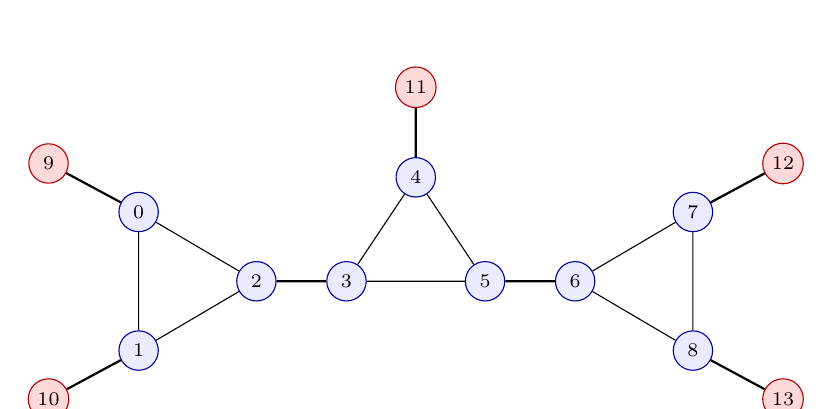
\begin{tikzpicture}[scale=.88,
 v/.style={circle,draw=blue!60!black,fill=blue!8,inner sep=2pt,minimum size=5mm,font=\scriptsize},
 b/.style={circle,draw=red!70!black,fill=red!15,inner sep=2pt,minimum size=5mm,font=\scriptsize}]
\node[v](a0)at(0,1){0};\node[v](a1)at(0,-1){1};\node[v](a2)at(1.7,0){2};
\node[v](a3)at(3,0){3};\node[v](a4)at(4,1.5){4};\node[v](a5)at(5,0){5};
\node[v](a6)at(6.3,0){6};\node[v](a7)at(8,1){7};\node[v](a8)at(8,-1){8};
\node[b](a9)at(-1.3,1.7){9};\node[b](a10)at(-1.3,-1.7){10};
\node[b](a11)at(4,2.8){11};\node[b](a12)at(9.3,1.7){12};\node[b](a13)at(9.3,-1.7){13};
\draw(a0)--(a1)--(a2)--(a0);\draw(a3)--(a4)--(a5)--(a3);\draw(a6)--(a7)--(a8)--(a6);
\draw[thick](a2)--(a3)(a5)--(a6)(a0)--(a9)(a1)--(a10)(a4)--(a11)(a7)--(a12)(a8)--(a13);
\end{tikzpicture}
\caption{The unique 14-vertex reduced equality graph at boundary five. Red
vertices are exactly the boundary. The labels agree with the Lean certificate
\texttt{Sharp14.lean}. Any bridge may be subdivided arbitrarily.}
\label{fig:sharp}
\end{figure}

\begin{proposition}[A degree constraint in the same class]\label{prop:degree}
Under the hypotheses of Theorem~\ref{thm:sharp},
\[
 \dd_G(x)+\ind_{\{x\in\bd G\}}\le b(G)\qquad(x\in V(G)).
\]
By Theorem~\ref{thm:unrestricted}, every five-boundary graph belongs to this
class. Thus every such graph has maximum degree at most five, and every
boundary vertex has degree at most four.
\end{proposition}
\begin{proof}
Each block satisfies
$\dd_B(x)+\ind_{\{x\in\bd B\}}\le b(B)$. This is immediate in case (i).
In case (ii), either every vertex is boundary, or there is one universal
interior vertex. That vertex has degree $b(B)$, and every other vertex is
nonuniversal and has degree at most $b(B)-1$.
For a non-cut vertex, use $b(B)\le b(G)$. At a cut vertex retain just the
incident blocks and its own defect in the nonnegative budget to obtain
\[
 b(G)\ge2+\sum_{B\ni x}(b(B)-2)+\delta_x
       =\sum_{B\ni x}b(B)-c_x+I_x\ge\dd_G(x)+I_x.
\]
\end{proof}

\section{The complete 227-kernel classification}
By Theorems~\ref{thm:budget} and \ref{thm:unrestricted}, every nonbridge
block of any five-boundary graph has diameter at most two. There is now
no restriction to a subclass. For consistency with the supplied initial
catalogue files, let $\mathcal C_2$ denote the class whose nonbridge
blocks have diameter at most two; all graphs considered here belong to it.

\begin{lemma}[The finite block palette]\label{lem:palette}
Exactly 24 nonbridge block types can occur in a connected graph with
boundary at most five. Their orders and intrinsic boundaries are:
\begin{center}
\begin{tabular}{@{}rrrl@{}}\toprule
Order & Boundary & Types & Description\\\midrule
3 & 3 & 1 & $K_3$\\
4 & 4 & 3 & $C_4$, $K_4$ minus an edge, $K_4$\\
5 & 4 & 2 & cones over $P_4$ and $C_4$\\
5 & 5 & 8 & all-boundary two-connected graphs of order five\\
6 & 5 & 10 & cones over connected order-five graphs with no universal vertex\\\bottomrule
\end{tabular}
\end{center}
The eight order-five cores are
\[
 C_5,\quad \Theta(1,2,3),\quad K_{2,3},\quad
 K_2\vee\overline{K_3},\quad K_{2,3}+e_3,\quad
 K_5-E(P_3),\quad K_5-e,\quad K_5.
\]
Here $e_3$ joins two vertices in the three-vertex part of $K_{2,3}$,
and $E(P_3)$ denotes two adjacent edges. The ten order-six cores are
$K_1\vee H$, where $H$ runs through the connected five-vertex graphs
of maximum degree at most three. These descriptions contain no boundary
predicate that still needs to be classified. The adjacency lists and
all stability values are in \texttt{small\_biconnected\_cores.json}.
\end{lemma}
\begin{proof}
The budget bounds the block boundary by five; the diameter-two theorem then
bounds its order by six. When there is an interior vertex, it is unique and
universal, so the graph is a cone. Two-connectivity is equivalent to connectivity
after deleting that vertex, and uniqueness says that the base has no universal
vertex. These facts give the listed descriptions. The remaining finite counts
were certified by enumerating all 33,864 labeled graphs of orders three through
six, with exhaustive degree-compatible permutation tests for isomorphism. This
checker is independent of the atlas and of nauty.
\end{proof}

\begin{remark}
Each boundary vertex in a two-connected cone with a unique universal vertex
has stability at least two. Indeed its base is connected, and every base vertex
$u$ has a nonneighbor at base distance two. Such a target has both the universal
vertex and a base neighbor as closer neighbors of $u$; all other neighbors are
at distance at most two. Hence the ten order-six/five-boundary cores admit no
boundary-preserving pendant attachment by Corollary~\ref{cor:exhaust}.
\end{remark}

\begin{figure}[p]
\centering
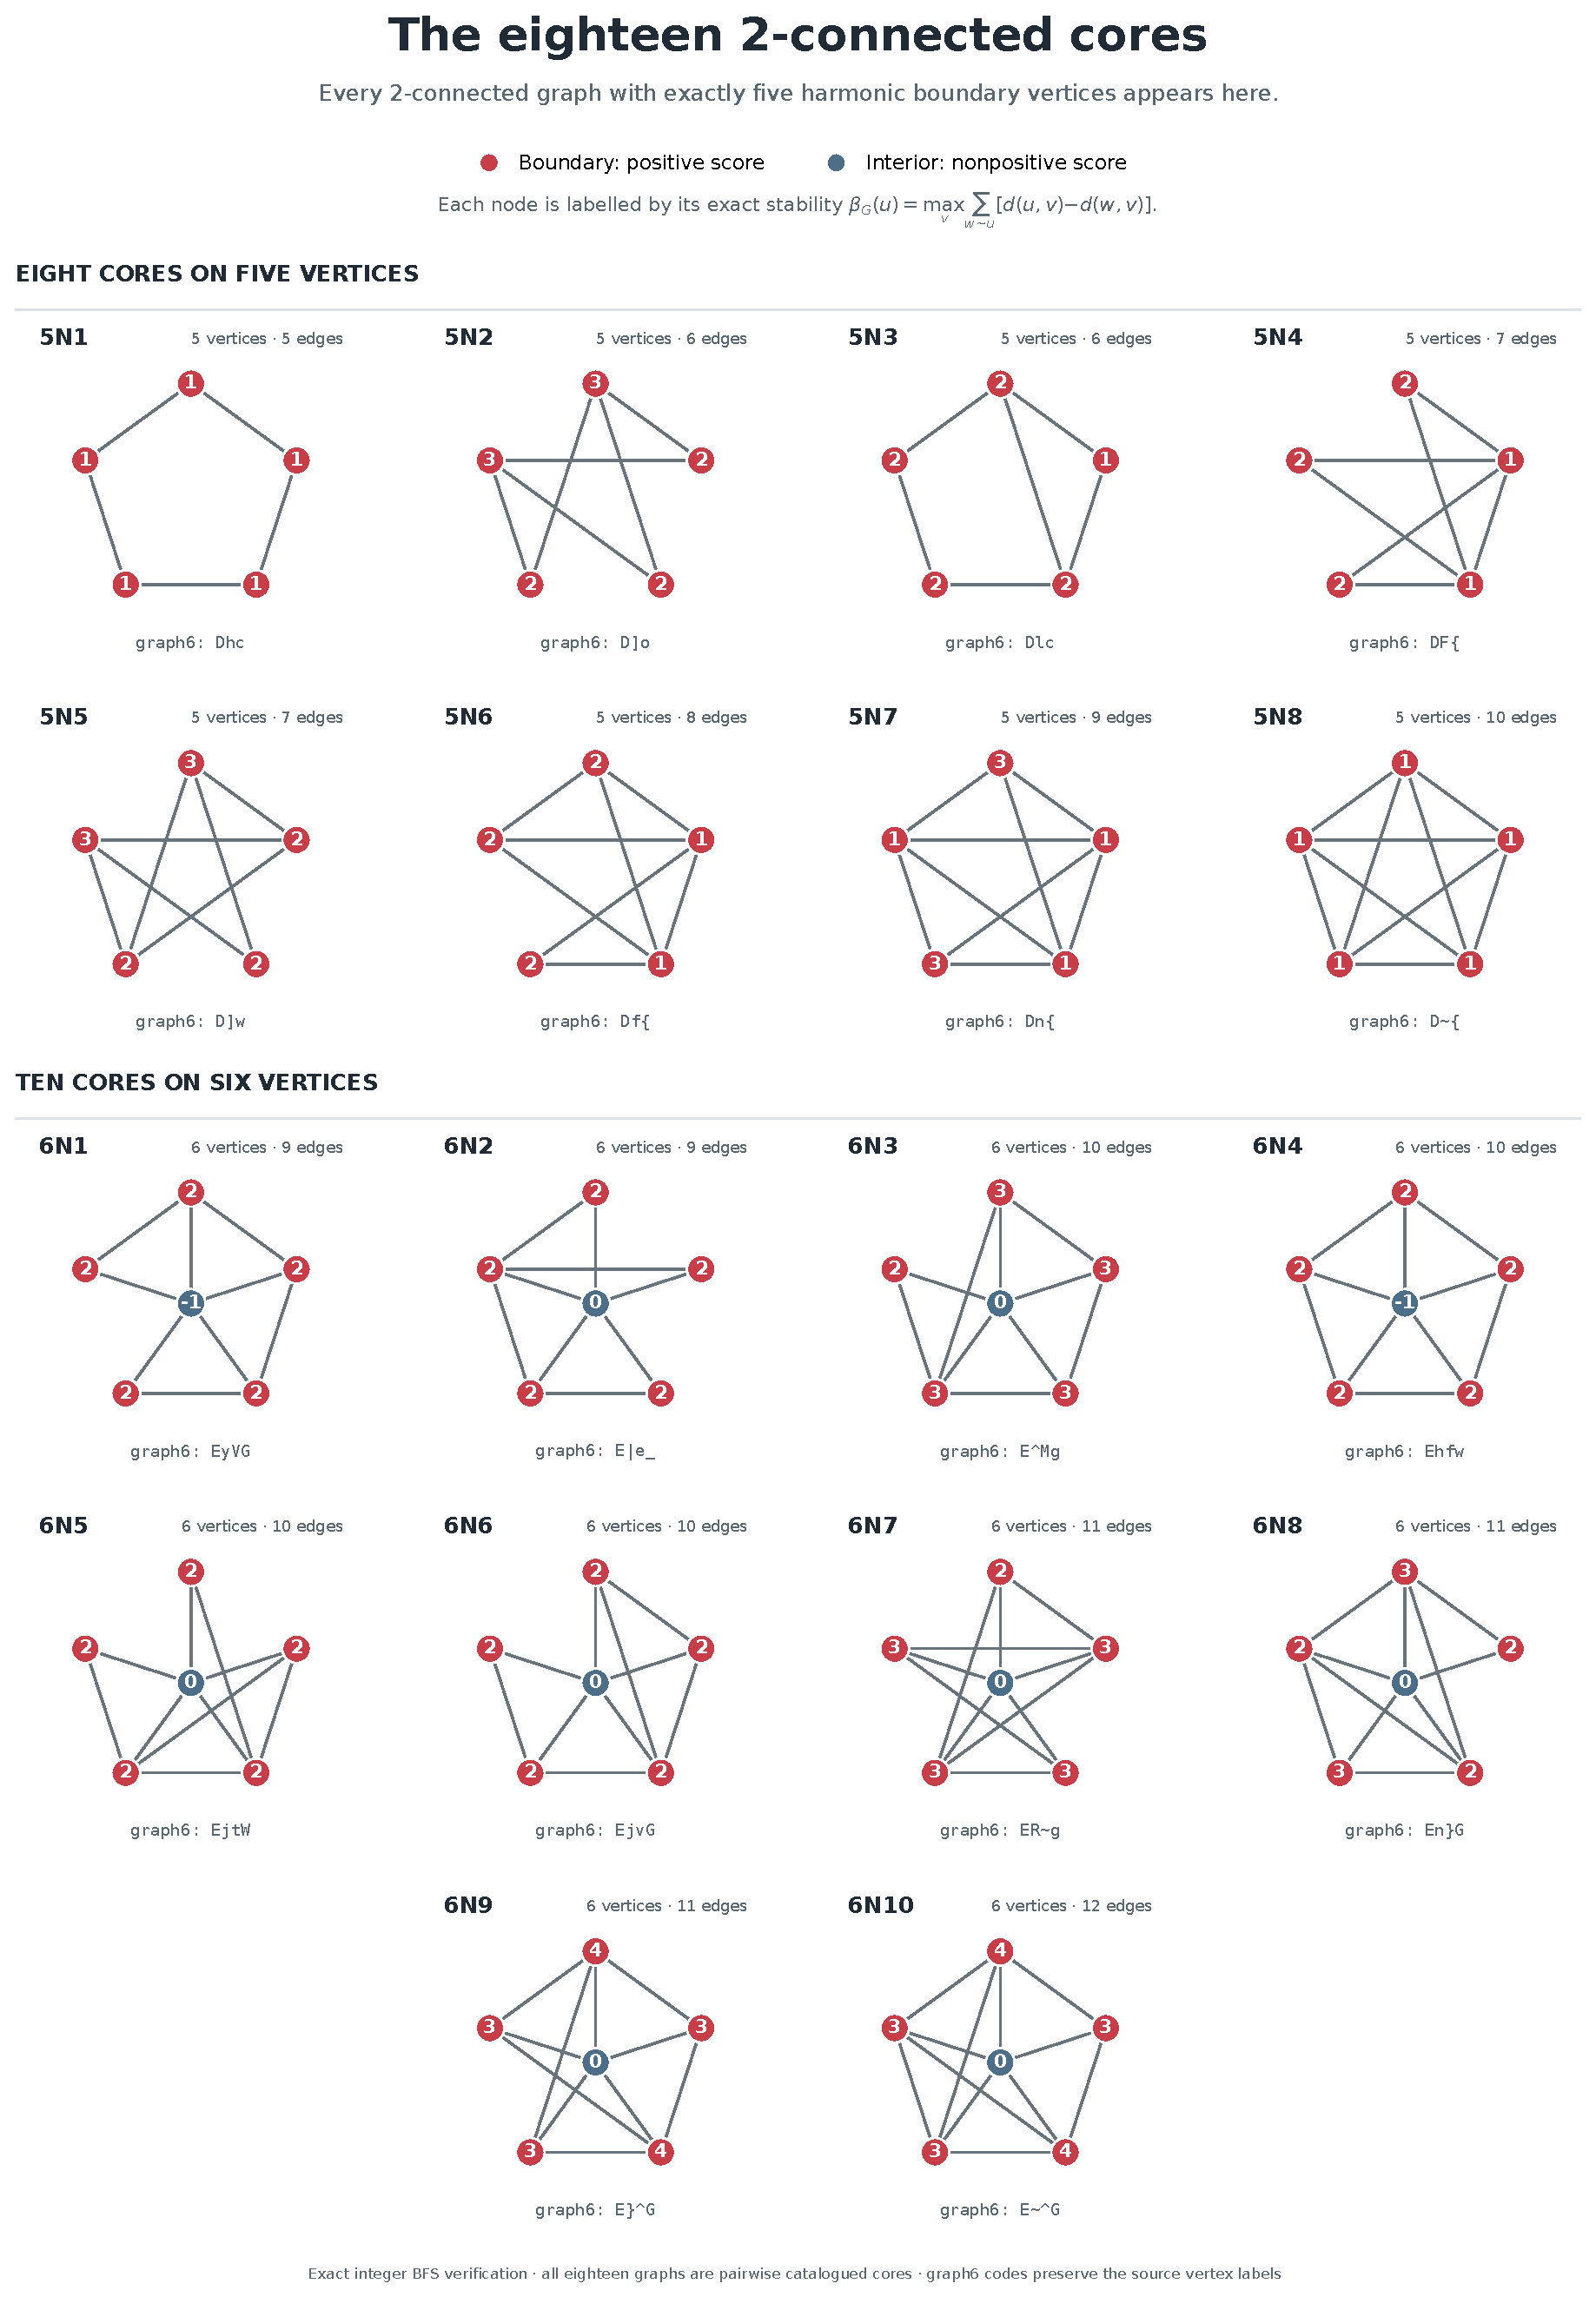
\includegraphics[width=\linewidth,height=.92\textheight,keepaspectratio]{figures/eighteen_cores.pdf}
\caption{All eighteen two-connected cores at boundary five. Vertex labels
are exact stability values, not vertex identifiers. Graph6 codes and the
full adjacency data are provided with the figure.}
\label{fig:eighteencores}
\end{figure}

\begin{theorem}[Exact finite classification]\label{thm:227}
A finite simple connected graph $G$ has five boundary vertices if and only if it is
obtained by independently subdividing bridges of one of the 227 pairwise
nonisomorphic graphs in \texttt{reduced\_kernels\_boundary5.g6}.
Their order distribution is
\begin{center}
\begin{tabular}{@{}lrrrrrrrrrrr@{}}\toprule
Order &5&6&7&8&9&10&11&12&13&14&Total\\
Kernels&10&33&34&42&41&34&19&10&3&1&227\\\bottomrule
\end{tabular}
\end{center}
The unique order-fourteen graph is Figure~\ref{fig:sharp}.
\end{theorem}
\begin{proof}[Mathematical completeness and finite verification]
Theorem~\ref{thm:sharp} bounds each reduced graph by 14 vertices, and
Lemma~\ref{lem:palette} gives its complete nonbridge palette. Include $K_2$ as
the bridge block. Starting from these 25 seeds, perform the following finite
closure: attach a rooted seed at a vertex of a current graph, or at a newly
inserted point inside one of its bridges; suppress any new degree-two bridge
vertex; retain boundary at most five; and identify isomorphic graphs.

This procedure is exhaustive, with single-block graphs as the induction base.
Remove an end block from a target reduced graph,
retaining its attachment vertex $x$. If a graph remains, it is connected and
stays in $\mathcal C_2$. Identifying graphs $A,B$ at a vertex gives
\[
 b(A\cup B)=b(A)+b(B)-I_A-I_B+I_{A\cup B}\ge b(A),
\]
because $b(B)\ge2$. Thus end-block deletion cannot increase the boundary.
Only $x$ can newly require suppression. Reversing deletion attaches the block
at an existing vertex or at a point in a bridge, exactly the two operations
above. Induction on the number of blocks proves completeness.

The computed closure contains 264 kernels with boundary at most five:
1, 5, 31, and 227 at boundaries 2, 3, 4, and 5. A second run without orbit
pruning reproduced the same set. A separate verifier used fresh breadth-first
distances and exact graph isomorphism, without nauty or the incremental
stability formula. It verified all seeds, pairwise nonisomorphism, and closure
under 7,788 attachment placements; all 3,194 placements retaining boundary at
most five were already in the catalogue. The completeness argument plus these
finite checks proves the count. Finally, bridge subdivision preserves the
boundary, completing both directions.
\end{proof}

\section{All five-boundary cacti}
For a cactus, every nonbridge block is a cycle. The intrinsic stability of every
vertex is one on an odd cycle and two on an even cycle. To see this, compare a
vertex with a target around the cycle: an even antipode has two closer
neighbors; an odd farthest target has one closer and one equidistant neighbor.
No target produces a larger value.

\begin{theorem}[Cactus boundary and exact classification]\label{thm:cactus}
The boundary of a cactus consists exactly of leaves, degree-two vertices on
cycles, and vertices incident with one even-cycle block and one bridge.
If
\[
 R_C=\sum_{\text{cycle blocks }C}(|C|-2),\qquad
 X=\sum_{x\in\cuts(G)}(t_x-2),
\]
and $E$ is the number of vertices meeting exactly one even cycle and one bridge,
then $b(G)=2+R_C+X+E$. Consequently the following is a complete
necessary-and-sufficient classification at boundary five:
\begin{center}
\begin{tabular}{@{}ll@{}}\toprule
Cycle multiset & Required attachment condition\\\midrule
No cycles & $X=3$ (trees with five leaves)\\
One triangle & $X=2$\\
Two triangles & $X=1$\\
Three triangles & $X=0$\\
One square & $X+E=1$\\
One pentagon & $X=0$\\
One triangle and one square & $X=0$, $E=0$\\\bottomrule
\end{tabular}
\end{center}
Every condition is computed on the actual cactus block tree. All bridge-path
lengths are arbitrary. Equivalently, there are exactly 121 reduced cactus
kernels, supplied in \path{cactus_reduced_kernels_boundary5.g6}.
\end{theorem}
\begin{proof}
A bridge block has intrinsic stability one at each endpoint. Combining these
values and the cycle values with \eqref{eq:block} gives the boundary list.
Every block vertex is intrinsically boundary, so $c_x=t_x$. The only globally
boundary cuts are the $E$ exceptional cuts, and
$\delta_x=t_x-2+I_x$. Equation~\eqref{eq:budget} gives the count.

The condition $R_C+X+E=3$ is necessary and sufficient. Since every cycle has
length at least three, partitioning $R_C\le3$ gives exactly the seven rows.
It also forces every cycle to have length at most five, so every five-boundary
cactus lies in $\mathcal C_2$. Selecting the cactus members of the complete
catalogue in Theorem~\ref{thm:227} gives 121 kernels.
\end{proof}

For clarity, the square row permits exactly one pendant path, or two pendant
paths at the same square vertex. The pentagon permits a single pendant path
at any chosen subset of its vertices. In the triangle-and-square row, the
cycles share one vertex directly; pendant paths may occur only at the other
two triangle vertices. The triangle-only rows are described without case
ambiguity by $X$. The unique 14-vertex kernel is a cactus, so the bound is
sharp already in this subclass.

\section{A sharp theorem for every two-tree}\label{sec:twotree}
A $k$-tree starts with $K_{k+1}$ and repeatedly adds a vertex whose neighbors
are the vertices of an existing $k$-clique. In particular, a two-tree is built
by adding triangle ears on edges. This section has no diameter restriction.

\begin{theorem}[Exact minimum boundary of a two-tree]\label{thm:twotree}
Among all two-trees on $n$ vertices, the minimum boundary cardinality is
\[
 \min b(G)=
 \begin{cases}
 3,&n=3,\\
 4,&n=4,5,\\
 \lceil n/2\rceil+2,&n\ge6.
 \end{cases}
\]
In particular, $n\le2b(G)-4$ for every two-tree of order at least six.
There are exactly three two-trees with five boundary vertices: the book of
three triangles $K_2\vee\overline{K_3}$, the cone over $P_5$, and the cone
over the five-vertex tree of degree sequence $(3,2,1,1,1)$.
\end{theorem}
The order bound is sharp at every even order, and its rounded boundary form
is sharp at every odd order as well. Maximality matters: there are
two-connected series-parallel graphs on nine vertices with boundary six,
so the same order bound does not hold for all partial two-trees.

\subsection{Localizing stability in chordal graphs}
A graph is chordal if it has no induced cycle of length at least four.
We use the elementary chordal facts that minimal vertex separators are
cliques and that a perfect elimination ordering can end in any specified
clique.

\begin{theorem}[Radius-two localization]\label{thm:local}
In every connected chordal graph,
\[
 \stab_G(u)=\max_{y:d_G(u,y)\le2}\stab_G(u,y).
\]
This identity concerns the maximum stability itself, not just its sign.
\end{theorem}
\begin{proof}
Let $y\notin N[u]$, let $C$ be its component in $G-N[u]$, and put
$S=N(C)\subseteq N(u)$. For every $s\in S$ a path $u,s,C,y$ avoids
$S\setminus\{s\}$, so $S$ is a minimal $u$--$y$ separator and is a clique.
There is a vertex $x\in C$ adjacent to all of $S$. For completeness, take
a perfect elimination ordering of $G[S\cup C]$ ending in $S$.
Deleting a simplicial vertex of $C$ preserves connectivity of the remaining
$C$, and preserves its full neighborhood $S$: a neighbor $s\in S$ of the
deleted vertex is also adjacent to its remaining neighbor in $C$.
The last vertex of $C$ is therefore complete to $S$.

Set $r=\min_{s\in S}d(s,y)$ and $A=\{s\in S:d(s,y)=r\}$.
Since $S$ is a clique, its other members have distance $r+1$.
Every path from $N(u)$ to $y$ enters $C$ through $S$. It follows that the
distances of vertices of $N(u)$ to $y$ are $r$ on $A$, $r+1$ on
$(N(u)\cap N[A])\setminus A$, and $r+2$ on $N(u)\setminus N[A]$.
As $d(u,y)=r+1$,
\[
 \stab(u,y)=|A|-|N(u)\setminus N[A]|
 \le |S|-|N(u)\setminus N[S]|=\stab(u,x).
\]
The final equality uses $N(x)\cap N(u)=S$, and $d(u,x)=2$.
\end{proof}

\begin{lemma}[Interior degree in a chordal graph]\label{lem:chordal-degree}
In a $k$-connected chordal graph, $k\ge2$, every nonuniversal interior
vertex has degree at least $2k+1$.
\end{lemma}
\begin{proof}
First $G[N(u)]$ is connected. A path in $G-u$ between two neighbors of $u$
can be shortened into $N(u)$, because each excursion through a component
of $G-N[u]$ enters and exits its clique separator.
Choose such a component, with separator $S$ of size $s\ge k$, and the
vertex $x$ complete to $S$ from the preceding proof. Put
$T=N(u)\cap N[S]$. Interiorness gives
$0\ge\stab(u,x)=s-\dd(u)+|T|$, so $\dd(u)\ge s+|T|$.
The set $S$ is proper in $N(u)$, since otherwise that score is positive.
Connectivity of $G[N(u)]$ gives $|T|\ge s+1$, proving the result.
\end{proof}

For an edge $ab$ of a two-tree, put $t_{ab}=|N(a)\cap N(b)|$.
The neighbor graph $G[N(u)]$ is a tree; the degree of its vertex $v$ is
$t_{uv}$. This follows directly by induction under triangle-ear addition.
Each exterior component has a separator which is an edge $ab$ of this tree;
such an attachment exists exactly when $t_{ab}\ge2$. Consequently
Theorem~\ref{thm:local} gives the exact formula
\begin{equation}\label{eq:local-two}
\stab(u)=\max\left\{
\begin{array}{ll}
2+t_{uv}-\dd(u)&(v\in N(u)),\\
2+t_{ua}+t_{ub}-\dd(u)&(uab\text{ a triangle},\ t_{ab}\ge2).
\end{array}\right.
\end{equation}
Indeed, the closed neighborhood of the edge $ab$ in the neighbor tree has
size $t_{ua}+t_{ub}$. A common exterior neighbor of $a,b$ gives the second
score; a neighboring target $v$ gives the first.

\subsection{Pruning and the sharp count}
\begin{lemma}[Pruning]\label{lem:pruning}
Let $G$ be a noncomplete $k$-tree, $k\ge2$, and remove any set $Q$ of
degree-$k$ vertices. If $H=G-Q$ has at least $k+2$ vertices, every
simplicial vertex of $H$ is a boundary vertex of $G$.
\end{lemma}
\begin{proof}
Degree-$k$ vertices of a noncomplete $k$-tree are independent and simplicial.
Their removal leaves a $k$-tree while at least $k+1$ vertices remain.
For a simplicial $u$ of $H$, the $k$-clique $S=N_H(u)$ extends in $H-u$
to a clique $S\cup\{x\}$. Thus $x\notin N_H[u]$ and $d_G(u,x)=2$.
Every removed neighbor $q$ of $u$ has its other $k-1$ neighbors in $S$.
Since $k\ge2$, $d_G(q,x)=2$. The $k$ vertices of $S$ are closer and
all other neighbors are equidistant, so $\stab_G(u,x)=k>0$.
\end{proof}
If the remainder is $K_k$, all its vertices are universal. If it is
$K_{k+1}$ and all its vertices were interior, a removed vertex $q$ omits
one core vertex $u$ and gives the same positive score $\stab_G(u,q)=k$.
These observations handle the small remainders below.

\begin{proof}[Proof of the lower bound in Theorem~\ref{thm:twotree}]
Suppose $n\ge6$, let $I=V\setminus\bd G$, let $i=|I|$, and write
$I_5=\{u\in I:\dd(u)=5\}$. Every interior vertex has degree at least
five, by Lemma~\ref{lem:chordal-degree}, or by $\dd(u)=n-1\ge5$
when it is universal.

We assign a distinct boundary vertex to every $u\in I_5$. Its neighbor
tree has five vertices. It cannot be a star, because the star center gives
a positive first score in \eqref{eq:local-two}. If the neighbor tree is
$P_5$, the second score says that only its two terminal edges can have
exterior attachments: an active edge's endpoint degrees must sum to at
most three. Its middle vertex $c$ therefore has global degree three.
If the neighbor tree is the fork of degrees $(3,2,1,1,1)$, only the edge
from the degree-two vertex to its leaf can have an exterior attachment.
The branching vertex $c$ has global degree four. In both cases $c$ is
boundary by Lemma~\ref{lem:chordal-degree}; assign it to $u$.

This assignment is injective. The two types cannot collide because their
assigned vertices have different global degrees. In the path case, write
the neighbor path as $a,b,c,d,e$. The only alternative interior neighbors
that could assign $c$ are $b,d$. In either of their neighbor trees, $c$
has degree one, rather than the degree two required of a path middle.
In the fork case, two other neighbors of the assigned branch have global
degree two. The sole remaining possible interior neighbor again sees
the assigned vertex with link degree one, rather than three.

Set $E_B=\sum_{v\in\bd G}(\dd(v)-2)$. Injectivity gives
$E_B\ge|I_5|$: path assignments use one unit, and fork assignments two.
The degree sum $4n-6$ now yields
\begin{equation}\label{eq:charge}
2(b-i-3)=E_B-|I_5|+
 \sum_{u\in I:\dd(u)\ge7}(\dd(u)-6)\ge0.
\end{equation}
Equality would force all assignments to be path assignments, and every
boundary vertex of degree greater than two to be an assigned degree-three
middle. Each such middle has three neighbors of degree greater than two:
its assigned interior root and its two neighboring vertices in the path.

Delete all degree-two vertices. They are independent, and the remainder
$H$ has at least two vertices, because each deleted vertex has two
undeleted neighbors. Every remaining boundary vertex still has degree
three in $H$. If $H$ is a noncomplete two-tree, its simplicial degree-two
vertex cannot be boundary, but cannot be interior by Lemma~\ref{lem:pruning}.
If $H=K_3$, all its vertices would be interior, excluded by the small-remainder
argument. If $H=K_2$, both vertices are universal and boundary, again
impossible. Equality in \eqref{eq:charge} is therefore excluded.
Its integer right side is even, hence at least two. Thus $b-i\ge4$,
and $n=b+i\le2b-4$.
\end{proof}

\subsection{Matching constructions and classification at five}
For $r\ge2$, start with a path $v_1,\ldots,v_r$ and independent vertices
$c_1,\ldots,c_r$. Join $c_j$ to $v_j$ and its available path neighbors
$v_{j-1},v_{j+1}$. This core is a two-tree. At each endpoint $v$, with
its corresponding $c$, choose either of the following three-vertex-end
configurations (the vertex $c$ is already present):
\begin{itemize}
\item add $p$ on $vc$, and then $q$ on $vp$;
\item add $p,q$ separately on $vc$.
\end{itemize}
Every $v_j$ has degree five; its neighbor tree is a path or the permitted
fork. Formula~\eqref{eq:local-two} gives $\stab(v_j)=0$.
Every other vertex has degree at most four and is boundary. Thus
$n=2r+4$ and $b=r+4$. The three unordered choices of endpoint types
give three equality examples for each $r\ge2$. The following sections prove
that these exhaust the even-order equality cases, classify all odd-order
cases, and give their exact unlabelled counts.
For $r=1$ the two appropriate choices give the cones over $P_5$ and
the fork, of order six. To obtain every odd order, use the first type at
both ends and add one ear on the outer edge $pq$. This activates only
a permitted terminal edge in the adjacent interior vertex's link.
The old $p,q$ have stability at least two, so remain boundary, and exactly
one new boundary vertex is added. This proves sharpness at every order.

At boundary five the bound forces $n\le6$. The two two-trees of order
five are the three-triangle book and the cone over $P_4$, of boundaries
five and four respectively. At order six there is one interior vertex;
its degree is five, so it is universal. A two-tree with a universal vertex
is the cone over a tree. The only five-vertex trees without a universal
vertex are $P_5$ and the fork. This proves the stated classification.

\begin{proposition}[All $k$-trees at boundary five]\label{prop:ktrees}
Every $k$-tree, $k\ge2$, satisfies
\[
 n\le(k+1)(b-k),
\]
with equality only for $K_{k+1}$. Across all $k\ge2$, the five-boundary
graphs are the three two-trees above, $K_5$ minus one edge (a three-tree),
and $K_5$ (a four-tree). For $k=1$ they are all trees with five leaves.
\end{proposition}
\begin{proof}
When $n\ge2k+2$, interior degrees are at least $2k+1$ and boundary
degrees at least $k$. The degree sum $2kn-k(k+1)$ gives the bound.
There are at least two boundary vertices of degree greater than $k$:
delete all degree-$k$ vertices and apply Lemma~\ref{lem:pruning} to the
two simplicial vertices of a noncomplete remainder. For a complete
remainder, at most one boundary core vertex would force every deleted
vertex to omit that same vertex, leaving at least two universal interior
vertices, a contradiction. Hence the large-order bound improves by two.

For $n\le2k+1$, minimum degree $k$ forces diameter at most two.
The known diameter-two theorem gives $b\ge n-1$. The cases
$n=k+1,k+2$ are a clique and a clique minus one edge; in the latter
there are at least two universal vertices and $b=n$.
For $n\ge k+3$,
$(k+1)(n-k-1)-n=kn-(k+1)^2\ge k-1>0$.
This proves the bound and its equality statement.
For $b=5$, it leaves $k=2,3,4$ and orders at most $9,8,5$.
Independent ear generation and recursive simplicial-degree-$k$
recognition on those finite ranges give exactly the five listed graphs.
The two-tree part has already been proved directly above.
\end{proof}


\section{Equality in the two-tree bound and quartic growth}
\label{sec:two-tree-equality-new}

Write $b=|\partial G|$, $i=|V(G)\setminus\partial G|$, and
$e=b-i-4=2b-|V(G)|-4$.  This section strengthens the sharp two-tree
bound $b\ge\lceil n/2\rceil+2$ for $n\ge6$.  Its most pronounced
consequence is a difference between the two parities.

\begin{theorem}[Complete equality grammars and growth]
Let $a_n$ be the number of isomorphism classes of two-trees on $n$ vertices
attaining $b=\lceil n/2\rceil+2$.
Then $a_6=2$ and $a_n=3$ for every even $n\ge8$.  At odd orders,
\[
 a_n\sim n^4/192.
\]
More explicitly, for every odd $n\ge19$,
\[
 a_n\ge \frac18\binom{(n-19)/2+4}{4}.
\]
All odd extremizers with noncomplete degree-two-pruned core are given by
an explicit finite grammar with $27$ states, $83$ productions, and $194$
terminal choices.  Exactly two additional complete-core examples occur,
both at order seven.  Every extremizer, of either parity, has maximum
degree at most six.
\end{theorem}

The exact rational generating function and period-eight formula are
proved in the subsequent exact-enumeration section.  The argument
below retains a separate proof of the quartic growth order.

The finite grammar is a necessary-and-sufficient description at every
order, rather than a list inferred from an initial census.  Its
graph-theoretic semantics are proved below; independent integer
checkers regenerate the complete state closure and certify the
pruning.  The grammar data are in
\texttt{checks/extensions/two\_tree\_equality/}.

\subsection{A structural defect identity}

Use the injective assignment from degree-five interior vertices to
boundary vertices established in the sharp-bound proof.  Path links
are assigned their degree-three middle and fork links their
degree-four branch.  Let $f$ count fork assignments and let $U$ be the
unassigned boundary vertices.  The exact degree identity is
\begin{equation}
 2e+2=f+\sum_{x\in U}(\deg x-2)
       +\sum_{\substack{x\notin\partial G\\\deg x\ge7}}(\deg x-6).
 \label{eq:new-defect}
\end{equation}
All terms are nonnegative.

Delete all degree-two vertices and call the resulting graph $H$.
If $H$ is noncomplete, it is a two-tree.  Every degree-two vertex of
$H$ is boundary in $G$, by the pruning lemma.  It cannot be an assigned
path middle, because all three neighbors of such a middle have
original degree greater than two.  Each core ear therefore consumes
at least one distinct unit of \eqref{eq:new-defect}.  Since $H$ has at
least two ears, this gives
\begin{equation}
 \begin{aligned}
 \#\{x:\deg_Hx=2\}&\le 2e+2,\\
 \deg_Gx&\le2e+6 &&(x\notin\partial G),\\
 \deg_Gx&\le\max(4,2e+3) &&(x\in\partial G).
 \end{aligned}
 \label{eq:new-structure}
\end{equation}
For the last bound, an unassigned boundary core ear leaves one unit
for another core ear; an unassigned boundary non-ear leaves two.
Assigned boundary vertices have degree at most four.

The triangle--edge incidence graph of a two-tree is a bipartite tree.
Remove its edge-nodes of degree one.  For noncomplete $H$, the leaves
of the remaining tree correspond exactly to its ears.  Thus its total
branching excess is at most $2e$.

There are elementary complete-core exceptions.  If $H=K_2$, all
vertices are boundary and $n=e+4$.  If $H=K_3$, write $p,q,r$ for the
numbers of attached ears on its three edges.  At least two numbers
are positive.  A core vertex is interior exactly when its opposite
multiplicity is zero and both incident multiplicities are positive.
Consequently, three positive multiplicities give $n=e+4$ and
$p+q+r=e+1$, all boundary; exactly two positive multiplicities give
$n=e+6$ and $p+q=e+3$, with one interior vertex.  Retain only cases
with $n\ge6$.  At $e=0$ this gives $(p,q,r)=(1,2,0)$, and at $e=1$
it gives $(1,3,0)$ and $(2,2,0)$, up to permutation.

\subsection{Even equality: precisely three strips}

At $e=0$, both units of \eqref{eq:new-defect} are consumed by two core
ears, so the internal incidence tree of $H$ is a path.  All interior
degrees are five or six and all boundary degrees are at most four.

For $r\ge2$, start with a path $v_1,\ldots,v_r$ and independent
vertices $c_1,\ldots,c_r$.  Join $c_j$ to $v_j$ and every existing
path neighbor of $v_j$.  At either endpoint $v$, with corresponding
$c$, choose a cap:
\begin{itemize}
\item $P$: add $p$ on edge $vc$, then $q$ on edge $vp$;
\item $F$: add $p$ and $q$ separately on edge $vc$.
\end{itemize}
These give $PP(r),PF(r),FF(r)$, with $2r+4$ vertices.  The $r$ path
vertices are interior of degree five; all others are boundary.  Their
numbers of degree-four boundary vertices are respectively zero, one,
and two, so they are pairwise nonisomorphic.

For completeness, process the triangle path $H$ from one end.  For
each active endpoint record current degree and accumulated local
boundary requirement, and record the final triangle multiplicity of
the active edge.  The exact local formula is
\begin{equation}
 \beta(u)=R_u-\deg u,\qquad
 R_u=\max\{2+t_{uv},\ 2+t_{ua}+t_{ub}:
                   uab\text{ a triangle},\ t_{ab}\ge2\}.
 \label{eq:new-local}
\end{equation}
Here $t_{uv}$ is the number of triangles on edge $uv$.  Requirements
can be capped at seven.  Forget a boundary vertex of degree three or
four with weight $+1$, or an interior vertex of degree five or six
with weight $-1$; each added ear has weight $+1$.  Accepted weight is
exactly $b-i$.

The complete closure has $18$ states and $58$ ordinary parameterized
transitions.  Exact prefix and suffix potentials show that weight
four paths use only these four states and arcs:
\[
\begin{array}{c|c|c|c}
 &((d_u,R_u),(d_v,R_v),t)&\text{initial}&\text{terminal}\\ \hline
A&((2,5),(3,4),2)&2&2\\
B&((2,5),(4,4),2)&-&1\\
C&((2,5),(3,5),2)&-&2\\
D&((2,5),(4,5),2)&3&1
\end{array}
\]
\[
 A\longrightarrow B\ (+1),\quad B\longrightarrow C\ (-1),\quad
 C\longrightarrow D\ (+1),\quad D\longrightarrow C\ (-1).
\]
The initial and final choices give the $P,F$ caps.  More explicitly,
in state $C$ the active edge is $(c_j,v_j)$ of degrees $(2,3)$.
The step to $D$ adds $v_{j+1}$, forgets $c_j$ as a degree-three boundary
vertex, and retains $(v_{j+1},v_j)$ of degrees $(2,4)$.  The return
step adds $c_{j+1}$, forgets $v_j$ as a degree-five interior vertex,
and retains $(c_{j+1},v_{j+1})$.  Thus the cycle is exactly strip
extension.  The two order-six exceptions are the cones over the
five-vertex path and the five-vertex fork.  This proves the full even
classification.

\begin{figure}[htbp]
\centering
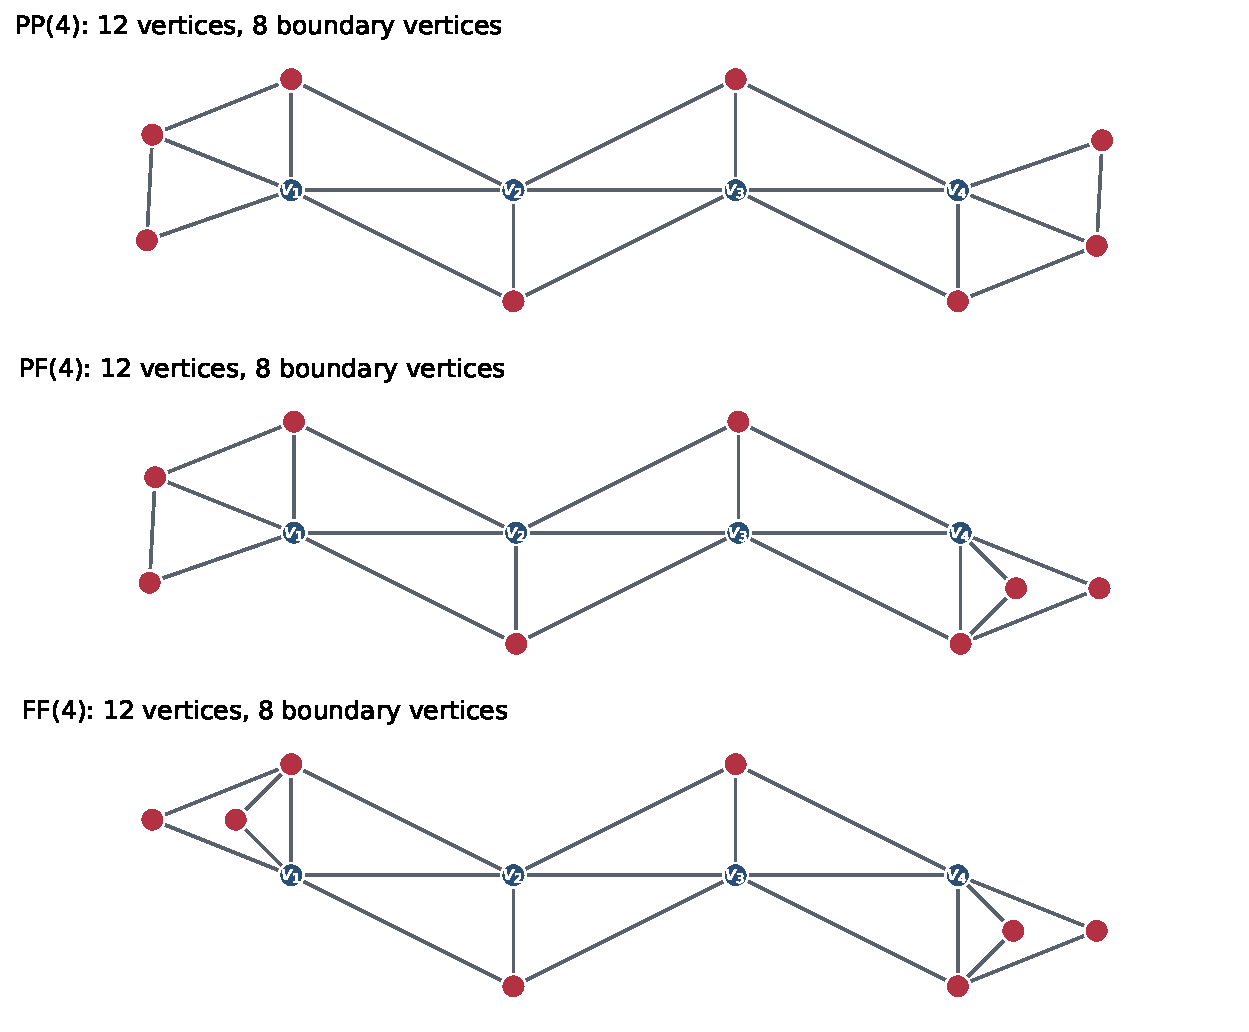
\includegraphics[width=.88\textwidth]{figures/even_extremal_families.pdf}
\caption{The three even extremal families at $r=4$. Blue vertices are the
four degree-five interior vertices; red vertices form the eight-point boundary.}
\end{figure}

\subsection{An exact rooted grammar at odd equality}

For $e=1$, \eqref{eq:new-structure} initially bounds interior degree
by eight, boundary degree by five, and core leaves by four.  A rooted
component has a pending root edge $uv$ and at least one outside core
triangle.  Its root ears are deferred.  If $k$ is the number of inside
core triangles on that edge, record at each endpoint a triple
$(d,A,B)$ whose requirement, at final root multiplicity $t\ge2$, is
\[
 \rho(t)=\max(A,B+t).
\]
The state is $(k;d_u,A_u,B_u;d_v,A_v,B_v)$, with endpoint triples
sorted.  Continuing degrees are at most seven; cap $A$ at nine and
$B$ at seven.  These caps preserve all decisions at final degree at
most eight.  A rooted component has one, two, or three leaves.

This information is sufficient: a forgotten vertex has every incident
edge closed.  Its only possible dependence on the pending root edge
is as the opposite edge of a triangle, whose active condition is
merely $t\ge2$ and is already fixed.  The two retained requirements
remain maxima of a constant and a constant plus $t$.

The operations are: an initial leaf triangle with ears on its closed
edges; adding one triangle and retaining a new root edge; joining
two components at a triangle; and identifying two pending root
edges.  In the last operation degrees add with subtraction of one,
because the root neighbor is counted twice, while $k,A,B$ combine by
addition, maximum, maximum, respectively.  In a triangle join, the
degree of the identified vertex is the sum of its child degrees
without subtraction.  All formulas follow directly from
\eqref{eq:new-local} and are given explicitly in the supplied note.
Final gluing identifies the two pending roots, adds any root ears,
and finalizes both endpoints.  Every forgotten vertex is required
to be boundary of degree three through five or interior of degree
five through eight.  Its sign, together with the ears, contributes
to component weight; the two pending roots are excluded.

Rooting the internal incidence tree at an internal edge yields two
components, each with at most three leaves.  Recursion into that
tree gives exactly the four operations.  This proves necessity;
the same interpretation and local formula prove sufficiency.
When the numerical root triples coincide, either physical ordering
is permitted: equal data do not imply a swapping automorphism.
No final productive equality state has such a tie.

The complete raw closure has $88,985,1153$ states with one, two,
three leaves, respectively.  It has nine initial, $126968$ binary,
and $6030$ unary productions.  Let $\mu(s)$ be the minimum component
weight.  The certified potentials satisfy, for every production,
\[
 \sum_j\mu(s_j)+w-\mu(s)\ge0.
\]
Rank-decreasing productivity witnesses attain every minimum.  A
minimum completed gluing is an actual graph and has weight at least
four.  Thus any accepted weight-five derivation has slack at most
one above its component minima.  Adding a slack coordinate $0$ or
$1$, retaining productive states, and tracing backwards from
weight-five terminal choices gives precisely $27$ states, $83$
productions, and $194$ terminal choices.  The two complete-core
exceptions at order seven finish the classification.

An independent verifier regenerates all raw rules and all $113830$
valid terminal gluings, checks $133007$ potential inequalities, and
checks the rank certificates and exact backward pruning.  A separate
program realizes all $4386$ productivity witnesses as actual graphs
and recomputes their full distance boundary scores by BFS.  Both
checks pass.  Every interior degree appearing in an accepted rule
or terminal choice is five or six.  This proves the claimed uniform
degree-six bound.

\subsection{Five strip parameters suffice}

The compact odd grammar has no triangle-join production.  Its pending
root multiplicities satisfy $k\le2$, and final root core multiplicity
is at most three.  Thus the internal core incidence tree branches
only at trivalent edge-nodes, with at most two branches.

Number the compact states from zero in the order in the data file.
The only cyclic strongly connected components of its unary part are
\[
 \{1,4\},\quad\{2,5\},\quad\{10,11\},\quad\{22,23\},
 \quad\{6\},\quad\{12\}.
\]
Each state has exactly one rule staying inside its cyclic component.
The two-step cycles insert a degree-five strip pair; the self-loops
insert a degree-six core vertex together with an ear.  Every complete
cycle has weight zero and adds exactly two vertices.

After contracting these components, the dependence graph is acyclic;
binary rules increase leaf count.  Consequently derivations consist
of finitely many templates, with one repetition parameter for each
cyclic component occurrence.  To count occurrences rather than just
topological core paths, assign to each contracted component $C$
\[
 M(C)=\mathbf1_{C\text{ cyclic}}+
 \max\Bigl\{\sum_j M(C_j):
    \text{a production enters }C\text{ from children outside }C\Bigr\}.
\]
The exact per-state vector is
\[
\begin{split}
(&0,1,3,0,1,3,2,0,1,2,4,4,3,3,0,2,\\
 &0,1,2,1,2,3,5,5,4,3,4).
\end{split}
\]
If the core branches, root at a trivalent edge-node, so the terminal
choice has $k_1+k_2=3$.  The maximum sum of these two state values is
five.  If the core is a path, root next to an end triangle: that side
is an initial leaf, with no repetition parameter, and the other side
has at most three.  Thus every odd extremizer has a finite-template
description with at most five nonnegative repetition parameters.
Each parameter adds two vertices, so at fixed order there are
$O(n^4)$ descriptions.  Ambiguity of descriptions can only reduce
the number of isomorphism classes.  This proves the upper bound.

\subsection{A matching five-parameter family}

Define a rooted arm $A(a)$, $a\ge0$, by taking a triangle $xyz$,
adding two ears on $xz$, adding $w$ on $yz$, and declaring the root
to be $(w,y)$, of degrees $(2,3)$.  Repeat $a$ times: on root
$(\ell,h)$ add $t$, then add $z'$ on $ht$, retaining root $(z',t)$.
This is compact state 1, of weight two and order $6+2a$.

Identify the low root endpoints and the high root endpoints of two
arms $A(a),A(b)$.  The resulting cherry $B(a,b)$ has root degrees
$(3,5)$, state 15, weight four, and order $10+2(a+b)$.
Starting with $B(c,d)$, add one vertex on its root edge and retain
the new vertex followed by the old low endpoint as root.  Its root
degrees are $(2,4)$, state 12, and weight three.  Repeat $r$ times:
add an ear and a continuing core vertex on this root edge, retaining
the new core vertex followed by the old low endpoint.  Each such
loop preserves state and weight and adds two vertices.

Finally identify this root crosswise with that of $B(a,b)$.  Both
final root endpoints have degree six and requirement six, so are
interior.  The resulting $F(a,b,c,d,r)$ satisfies
\[
 |V(F)|=19+2(a+b+c+d+r),\qquad b(F)-i(F)=4+3-2=5.
\]
It is therefore extremal for every nonnegative choice of parameters.

Its canonical degree-two-pruned core incidence tree has two trivalent
edge-nodes.  The four pendant paths contain $2+2a,2+2b,2+2c,2+2d$
triangle-nodes, in pairs at the two branches.  The path between the
branches contains $r+1$ triangle-nodes.  An isomorphism thus
determines $r$ and the unordered pair $\{\{a,b\},\{c,d\}\}$.  At
most eight ordered tuples can describe one isomorphism class.
For sum $S$, there are $\binom{S+4}{4}$ tuples, yielding the stated
lower bound.  Combined with the upper bound, this proves
$a_n=\Theta(n^4)$ through odd $n$.

The recovered incidence-tree lengths are graph invariants, as
shown above.  As a numerical check, all $792$
tuples of sum at most seven, reaching order 33, pass fresh BFS
boundary checks and exact parameter recovery.  The subsequent section
strengthens this result to an exact generating function and leading
coefficient by resolving all isomorphism identifications.

\subsection{Finite-state classification at every fixed excess}

\begin{theorem}[Effective fixed-excess grammar]
For each fixed integer $e\ge0$, the two-trees of order at least six
with $2b-n-4=e$ are generated by an effectively constructible finite
grammar, together with the explicit complete-core cases above.
Put $C=2e+6$, $L=2e+2$, and $K=(C-2)^2(C-1)$.  The grammar needs
at most
\[
 (e+1)(L-1)^2\frac{K(K+1)}2=O(e^9)
\]
states.
\end{theorem}

\begin{proof}
Use \eqref{eq:new-structure} and the same rooted requirements
$\max(A,B+t)$.  A continuing endpoint has degree in $[2,C-1]$;
cap $A$ at $C+1$ and $B$ at $C-1$.  Since $t\ge2$, both caps
preserve all boundary comparisons.  The endpoint triples thus
have $K$ possible numerical values.  The inside root multiplicity
and leaf count both lie in $[1,L-1]$.  Sorting the two triples gives
at most $(L-1)^2K(K+1)/2$ raw state/leaf pairs.  Ear multiplicities
are also bounded by degree.  The four operations and final gluing
remain exact, and cover every core of at most $L$ leaves.

Every reachable component weight is bounded below.  Indeed, fill its
pending root with one outside triangle and no root ears.  Previously
forgotten statuses are unchanged because root multiplicity remains
at least two.  The completed two-tree has weight at least four at
order at least six, and at least three at smaller orders.  Its two
former roots and new vertex contribute at most three.  Thus all
component weights are nonnegative, and state minima are attained
integers.  They can be computed by increasing leaf count: binary
joins use smaller counts and unary extensions give a finite
shortest-path problem without reachable negative cycles.

Reduced production costs are nonnegative.  Every minimum completed
gluing is an actual graph of weight at least four, so for target
$e+4$, each subcomponent's slack is in $[0,e]$.  Adjoining this
budget coordinate, retaining productive states, and accepting
exact total weight $e+4$ yields the claimed finite grammar and state
bound.  The complete-core cases have already been classified.
\end{proof}

This theorem does not assert polynomial unlabelled growth at every
fixed excess.  The deterministic cyclic structure required for the
quartic statement was certified specifically for $e=1$.

\paragraph{Formal verification scope.}
The Lean file \texttt{EvenEqualityAutomaton.lean} proves that every
accepted run, of arbitrary length, has weight at least four and
that every weight-four run uses only the four optimal transitions.
The odd finite grammar is also accompanied by a universal
derivation-weight and interior-degree certificate.  The
graph-to-state correspondence, core reduction, and counting
argument are ordinary mathematical proofs supported by independent
exact checkers; they are not claimed as end-to-end Lean
formalizations.

\section{Exact enumeration: a rational function and a period-eight formula}
\label{sec:exact-odd-count}

The finite grammar can be made unambiguous by using the canonical
degree-two-pruned core.  This gives an exact count, strengthening the
quartic growth theorem.

\begin{theorem}[Exact unlabelled equality count]
There is one minimum-boundary two-tree at each of orders three,
four, and five, namely $K_3$, $K_4-e$, and the cone over $P_4$.
There are two at order six, seven at order seven, and exactly three
at every even order at least eight.  For every odd $n\ge9$,
\[
 a_n=\frac{n^4-20n^3+239n^2+c_rn+d_r}{192},\qquad r=n\pmod8,
\]
where
\[
\begin{array}{c|rrrr}
r&1&3&5&7\\ \hline
c_r&-1126&-1090&-1126&-1090\\
d_r&2250&1962&2298&1914
\end{array}
\]
In particular $a_n\sim n^4/192$ through odd $n$.
With $t=x^2$, the exact generating function is
\begin{equation}
 \sum_{\substack{n\ge7\\n\text{ odd}}}a_nx^n
 =\frac{x^7N(t)}{(1-t)^5(1+t)^2(1+t^2)},
 \label{eq:exact-count-gf}
\end{equation}
where
\[
 N(t)=7-3t-4t^2+8t^3-t^4+4t^5+11t^6-8t^7+t^8+t^9.
\]
\end{theorem}

\subsection{Canonical arms and their generating functions}

Use the state numbering of the compact odd grammar.  For
$j=0,\ldots,9$, let $F_j(x)$ count rooted component isomorphism
classes in state $j$, with $x$ marking vertices other than its two
root endpoints.  These are one-leaf components, so their pruned
core is a triangle path.  Their root endpoint triples are unequal
and fix an orientation.

There is a unique decomposition of such a rooted graph.  Retain
the two marked root endpoints and remove every other degree-two
vertex; this recovers its rooted core.  Its root triangle either
is the sole triangle, or has exactly one continuing core edge.
The ear multiplicities and the continuing edge determine the
last extension uniquely, including the predecessor orientation.
Iterate towards the leaf.  The only duplicate initial parameters
are $(p,0)$ and $(0,p)$ for $p=1,2,3$, which describe the same
canonically oriented cap and are counted once.  Thus the unary
transition equations are exact unlabelled equations, rather than
equations for derivations.  Their solutions are
\[
\begin{array}{c|l@{\qquad}c|l}
j&F_j(x)&j&F_j(x)\\ \hline
0&x^2&5&x^4(1+4t-3t^2)/(1-t)^3\\
1&2x^4/(1-t)&6&2x^5/(1-t)^2\\
2&x^3(1+4t-3t^2)/(1-t)^3&7&x^4\\
3&x^3&8&2x^4(1+t)/(1-t)\\
4&x^3(1+t)/(1-t)&9&x^4(1+t^2)/(1-t)^2
\end{array}
\]
These identities follow from all one-leaf rules with the three
initial seeds $F_0=x^2$, an added $x^3$ in $F_4$, and an added
$x^4$ in $F_9$.  Every extension increases order, so the solution
as formal power series is unique.

Define
\[
 A=F_0+F_1=\frac{x^2(1+t)}{1-t},\qquad
 B=F_3+F_4+F_6=\frac{2x^3}{(1-t)^2}.
\]
The $A$-arms have weight two and root degrees $(2,3)$; the
$B$-arms have weight three and root degrees $(2,4)$.  For an
unlabelled class $C$, unordered pairs have generating function
\[
 \operatorname{Pair}(C)(x)=\frac{C(x)^2+C(x^2)}2.
\]
Set
\[
 M=\operatorname{Pair}(A)
   =\frac{x^4(1+t+2t^2)}{(1-t)^2(1+t)}.
\]

\subsection{One or two branches}

If the core has one branch, its unique trivalent edge-node
canonically roots the graph.  Each arm has low root degree two
and high root degree at least three.  One root ear would make
the sum of final root degrees at least $3\cdot5-4+2=13$, so
there are no root ears.  No endpoint can be high in all three
arms, which would give degree at least seven.  Each therefore
has requirement at least six.  The degree sum is at least
eleven; degrees five and six would give one boundary and one
interior root, and weight at least six.  Hence both root
endpoints are interior of degree six.  The three arm
weights must be $2,2,3$.  The endpoint degree equations force
the weight-three arm to have root degrees $(2,4)$, and the
two weight-two arms to have their degree-three sides aligned
with its degree-two side.  Thus there are two $A$-arms and one
$B$-arm.  The unique $B$-arm fixes the root ordering, and the
$A$-arms form an unordered pair.  Every such combination has
requirement six at both final endpoints.  Therefore the exact
three-leaf contribution is
\begin{equation}
 U_3=x^2MB
 =\frac{2x^9(1+t+2t^2)}{(1-t)^4(1+t)}.
 \label{eq:count-u3}
\end{equation}

With two branches, the same root equations force two $A$-arms
at each branch and state 12 for the component leading to the
other branch.  The only entries into state 12 are an extension
of states 14 or 15, which are a pair of $A$-arms, and its
degree-six self-loop.  Hence the graph is determined by an
unordered pair of unordered pairs of $A$-arms, and a central
length $r\ge0$.  The core canonically recovers all these data.
Reversing the central strip exchanges its two branches: the
central core is the square of a path, with one ear on each
strictly internal consecutive edge, and the higher arm-degree
endpoint at the outer end of either terminal edge.  This
reversal preserves the endpoint roles for every $r$.
Consequently the exact four-leaf contribution is
\begin{equation}
 U_4=\frac{x^3}{1-x^2}\operatorname{Pair}(M)
 =\frac{x^{11}(1+4t^2+2t^3+6t^4+3t^6)}
 {(1-t)^5(1+t)^2(1+t^2)}.
 \label{eq:count-u4}
\end{equation}
The canonical decomposition proves that repeated or equal arms
are counted correctly; there is no assumption that grammar
derivations are unambiguous.

\subsection{Path cores and reflection}

For a path core, mark one of its two end triangles.  Its core
ear and opposite internal edge are intrinsic.  Exactly one
closed edge of this end triangle has ears, so this fixes the
root endpoint order.  The end component is a literal initial
cap in state 0,4, or9.  The terminal table with this cap first
and its orientation zero gives the end-rooted function
\begin{align*}
 E={}&x^4(F_2+2F_3+2F_4+F_6)\\
 &+x^5(3F_0+3F_1+F_5+F_7+F_8+F_9)\\
 &+x^6(2F_3+2F_4+F_6)\\
 ={}&\frac{4x^7(2+t-3t^2+t^3)}{(1-t)^3}.
\end{align*}
Selecting the other end is an involution.  Its fixed classes
are exactly graphs admitting an end-exchanging automorphism.
If their generating function is $S$, Burnside's elementary
two-element formula gives $U_2=(E+S)/2$.

The center of the core incidence path is an edge-node or a
triangle-node.  Its symmetry cases are exhaustive as follows;
$q$ counts ears on the central edge, or on each of the two
internal edges at a central triangle.
\[
\begin{array}{c|c|l|c}
\text{center}&\text{half states}&\text{matching}&q\\ \hline
\text{edge}&0,1&\text{same endpoint order}&1\\
\text{edge}&3,4,6&\text{opposite endpoint order}&1\\
\text{triangle}&0,1&\text{shared corner high}&0\\
\text{triangle}&3,4&\text{shared corner low}&0\\
\text{triangle}&3,4,6&\text{shared corner low}&1
\end{array}
\]
Here ``low'' and ``high'' refer to the half's two root degrees.
At an edge center the weight equation is
$2w+q+s_u+s_v=5$, so parity forces $q=1$; the root degree and
requirement tests give the first two rows.  At a triangle
center, let $u$ be the shared corner and $v,w$ the exchanged
corners.  Initially allow $r$ ears on the third edge.  Then
$D_u=2d_u+2q$, $D_v=D_w=d_v+q+1+r$, and the weight is
$2w+2q+r+s_u+2s_v$.  The degree bound gives $q\le1$.
If $r>0,q=1$, the shared corner would have degree six and
requirement at least eight, impossible.  If $r>0,q=0$ and
the shared corner is high, the other two corners are boundary
and the weight is at least $4+r+1\ge6$.  If the shared corner
is low, it is boundary.  Half high degree three then gives
weight at least eight; high degree four allows only $r=1$
and gives weight at least six; larger degrees are impossible.
Thus $r=0$.  The degrees reduce to
$D_u=2d_u+2q$ and $D_v=D_w=d_v+q+1$, and the weight equation is
$2w+2q+s_u+2s_v=5$.  If $u$ is low, its requirement is $5+q$,
and that at $v$ is $\max(A_v,5+q)$.  If $u$ is high, the
degree-six bound forces high degree three and $q=0$.  These
conditions give exactly the remaining three rows.

Isomorphic rooted halves always give the required reflection;
use an isomorphism in one direction and its inverse in the
other.  Conversely every end exchange identifies the halves
in one listed way.  Unequal root summaries preclude another
root-swapping identification within a half.  The center type
and its ear multiplicities are intrinsic, so the cases are
disjoint.  Doubling the half replaces $x$ by $x^2$, giving
\begin{align*}
 S_{\rm edge}&=x^3(F_0+F_1+F_3+F_4+F_6)(x^2),\\
 S_{\rm triangle}&=x^3(F_0+F_1+F_3+F_4)(x^2)
                  +x^5(F_3+F_4+F_6)(x^2),\\
 S&=\frac{2x^7(1+t-t^3)}{(1-t)^2(1+t)}.
\end{align*}
Thus
\begin{equation}
 U_2=\frac{x^7(5+6t-5t^2-5t^3+3t^4)}{(1-t)^3(1+t)}.
 \label{eq:count-u2}
\end{equation}
The path-core count is five at order seven and, for odd $n\ge9$,
equals $(n^2-25)/4+\lfloor(n+1)/4\rfloor$.

\subsection{Exact algebra and independent checks}

The complete-core exceptions contribute $2x^7$.  The other
classes have respectively two, three, and four core leaves,
so are disjoint.  Adding $2x^7+U_2+U_3+U_4$ yields
\eqref{eq:exact-count-gf}.

To certify the quasipolynomial without extrapolation, put
$m=(n-7)/2=4k+r$.  Its four Newton coefficient rows, indexed
by $r=0,1,2,3$, are
\[
\begin{array}{c|rrrrr}
0&8&109&502&896&512\\
1&18&177&678&1024&512\\
2&36&280&886&1152&512\\
3&66&420&1126&1280&512
\end{array}
\]
The corresponding polynomial is
$P_r(k)=\sum_{j=0}^4c_{rj}\binom{k}{j}$; subtract one only
at $m=0$.  Since
$\sum_{k\ge0}\binom{k}{j}z^k=z^j/(1-z)^{j+1}$, these rows
give a rational function with denominator $(1-t^4)^5$.
Cross-multiplication with \eqref{eq:exact-count-gf} is an
exact integer polynomial identity.  Expanding the four
polynomials in $n$ proves the displayed residue formula for
every odd $n\ge9$, with $a_7=7$ as its sole initial correction.

The standard-library checker \texttt{exact\_odd\_count.py}
verifies every one-leaf recurrence, terminal sum, symmetry
formula, unordered-pair identity, and the exact polynomial
certificate.  A separate program of the earlier session generates the complete
grammar by increasing order and canonicalizes graphs using
recursive ordered-edge incidence codes.  Equality of these
codes is exact equality of recursive tuples; rerooting at
all edges and both orders gives unlabelled isomorphism.
It reproduces every individual nauty class through order 13
and all stratified counts through order 35, where there are
$4686$ extremizers.  These experiments check the all-order
canonical proof rather than replace it.  The counting
correspondence is not represented as an end-to-end Lean
formalization.  The exact integer-polynomial identities for
the summed numerator and Newton coefficient formula are
separately kernel-checked in
\texttt{OddCountingIdentities.lean}.

\section{Rational enumeration at every fixed excess}
\label{sec:fixed-excess-rationality}

The fixed-excess grammar can be strengthened to an effective rational
enumeration theorem.  The proof counts canonical colored incidence
trees, rather than ambiguous grammar derivations.

\begin{theorem}[Rational unlabelled enumeration at fixed excess]
\label{thm:fixed-excess-rationality}
Fix an integer $e\ge0$, and let $\mathcal C_e$ be the isomorphism
classes of two-trees $G$ of order at least six with
$2|\partial G|-|V(G)|-4=e$.  Then
\[
 F_e(z)=\sum_{[G]\in\mathcal C_e}z^{|V(G)|}
\]
is an effectively computable rational function.  In particular,
for each fixed $e$, its exact unlabelled counts eventually satisfy
a constant-coefficient linear recurrence.
\end{theorem}

The restriction to orders at least six avoids the exceptional small
orders in the sharp bound.  Extending a fixed-excess count to all
orders changes its generating function by only a finite polynomial.
No practical complexity bound is asserted for the general algorithm.

\subsection{Finite bounds and an intrinsic pending-root weight}

Put
\[
 C=2e+6,\qquad D=\max(4,2e+3),\qquad L=2e+2.
\]
The structural defect theorem bounds interior degrees by $C$ and
boundary degrees by $D$.  Remove all degree-two graph vertices to
obtain the canonical core $H$.  If $H$ is noncomplete, it is a
two-tree with at most $L$ ears.  Its internal triangle--edge incidence
tree, obtained by deleting private edge-nodes, has at most $L$
leaves.  Every removed vertex is an ear on a core edge $f$; write its
multiplicity as $q_f$.  Since each core endpoint has degree at least
two in $H$,
\[
 0\le q_f\le C-2.
\]
The complete cores $K_2,K_3$ have the already classified orders
$e+4$ or $e+6$ and bounded ear multiplicities, so contribute a
finite polynomial.  We treat noncomplete cores below.

Cut at an internal core edge $uv$, with at least one core triangle
on either side, and defer all ears on that root edge.  Exclude
$u,v$ from the component weight $W$.  Every other vertex receives
its boundary/interior sign under the \emph{pending-root convention}
that the final multiplicity of $uv$ is at least two.  This is not
the raw boundary weight of the isolated component.  Indeed, adding
the first outside triangle can activate a local condition at a page
vertex.  Under the pending convention that condition is already
active: the local formula
\[
 \beta(u)=R_u-\deg u,\quad
 R_u=\max\{2+t_{uv},\ 2+t_{ua}+t_{ub}:
 uab\text{ a triangle},\ t_{ab}\ge2\}
\]
depends on the root edge, for a nonroot vertex, only through the
threshold $t_{uv}\ge2$.  All incident edges and degrees of that
nonroot vertex are closed.  Thus $W$ is intrinsic and independent
of the chosen completion with an active root edge.

Every such component of a graph in $\mathcal C_e$ satisfies
\begin{equation}
 0\le W\le e+6.
 \label{eq:rational-pending-weight}
\end{equation}
To prove the lower bound, add one vertex on the root edge.  Its
multiplicity is now at least two, preserving exactly the pending
nonroot signs just defined.  Every two-tree of order at least three
has total boundary-minus-interior weight at least three, by the
sharp theorem and the direct small-order check.  This completion
has at least four vertices, so a convention also admitting $K_2$
is irrelevant.  Its two former roots and new degree-two vertex
contribute at most three, proving $W\ge0$.

For the upper bound, let $W'$ be the pending nonroot weight of the
complementary component, and $q$ the root ear multiplicity.  With
root signs $s_u,s_v\in\{-1,1\}$, the final graph gives
\[
 e+4=W+W'+q+s_u+s_v.
\]
Since $W'\ge0$, $q\ge0$, and $s_u+s_v\ge-2$, the upper bound in
\eqref{eq:rational-pending-weight} follows.  The argument also
applies to any nonempty proper group of pages at an internal edge.

\subsection{An exact finite-alphabet incidence encoding}

A two-tree has a proper three-coloring unique up to one global
permutation: name the colors on an initial triangle, after which
each added vertex is forced to use its two parents' missing color.
For a named coloring of $H$, color every edge-node of its full
triangle--edge incidence tree by the missing endpoint color.  The
three edge-nodes at a triangle have different colors.  This colored
tree reconstructs the colored graph uniquely.  Root at a triangle,
name its three vertices by color, and traverse the tree; every new
triangle shares a known edge and introduces one new vertex of the
missing color, while its two other edge colors determine the
incidences.  Conversely this procedure reconstructs a two-tree
from every locally valid such colored incidence tree.

Use the internal incidence tree $T$, obtained by deleting all
edge-nodes lying in just one triangle.  Give its nodes finite labels:
\begin{itemize}
\item an internal edge-node carries its missing color and $q_f$;
\item a triangle-node records the subset of edge colors remaining
internal, and the ear multiplicity for each missing private edge
color.
\end{itemize}
Its neighboring edge colors must be precisely that recorded subset.
All deleted private edges can be restored uniquely.  Thus these
labels reconstruct $H$ and then $G$.  Ears on one edge are represented
by their multiplicity, so their permutations are already removed.

The alphabet is finite.  Triangle degrees are at most three, and
edge-node degrees are at most $L$, since $T$ has at most $L$ leaves.
All leaves are triangle-nodes.  Define a node weight by
\[
 \omega(v)=
 \begin{cases}
 1+\sum q_f,&v\text{ a triangle-node, over its private edges},\\
 q_f,&v\text{ an internal edge-node}.
 \end{cases}
\]
Then
\begin{equation}
 |V(G)|=2+\sum_{v\in T}\omega(v).
 \label{eq:rational-node-weight}
\end{equation}
A core with $t$ triangles has $t+2$ vertices, and every ear has been
counted once.  All weights are nonnegative and triangle weights
are positive.  Color permutations preserve them.  Colored decorated
tree isomorphism is exactly colored graph isomorphism; forgetting
colors adds precisely the one global $S_3$ action, with no separate
gluing gauge at each edge.

\subsection{A deterministic recognizer on the canonical tree}

Root $T$ at a designated leaf triangle.  At an internal edge cut,
order the two graph endpoints by their named colors and retain:
the number of inside root triangles; both current endpoint degrees;
both requirements $\max(A,B+t)$, with $A$ capped at $C+1$ and $B$
at $C-1$; the inside leaf count; actual pending weight $W$ in
$\{0,\ldots,e+6\}$; and the finite deferred-ear and color data.
Continuing degrees are at most $C-1$.  The requirement caps preserve
every final comparison at degree at most $C$, since $t\ge2$.
All coordinates are finite; include a rejecting state.

There are canonical deterministic transitions.  A triangle has zero,
one, or two active child core edges, whose ports are distinguished
by color.  The local boundary formula computes the affine root
requirements and the final sign and degree of its third vertex;
labels specify all ear multiplicities.  Add that sign and the ears
to $W$.  At an edge-node combine \emph{one unordered star of all
child triangle branches at once}: root degrees add with subtraction
for the repeated root neighbor, requirements combine by maxima,
and triangle counts, leaves, and nonroot weights add.  This transition
is symmetric in a bounded multiset of child states, retaining the
full multiplicity of repeated branches.  No binary-join history is
counted.  The affine constants can be defined intrinsically as
maxima of constant and root-linear local contributions, rather
than by a choice among equivalent formulas.

Require each finalized retained core vertex to have degree at least
three and satisfy the appropriate boundary/interior cap.  Reject if
any state bound is exceeded.  At the root leaf triangle, close the
remaining edge, account for its ears and the two private edges,
finalize all remaining vertices, and accept exactly at total weight
$e+4$.  The root core vertices must also finish with degree at least
three.

Every member of $\mathcal C_e$ passes under any chosen leaf root,
by the proved bounds and exact local formula.  Conversely an accepted
decorated tree reconstructs a two-tree whose specified core vertices
all have degree at least three and whose attached ears have degree
two.  Its specified core is therefore the canonical pruned core.
All signs are correct and total weight $e+4$ is exactly the desired
excess.  A noncomplete pruned core with all ears retained above degree
two gives order at least six.  Thus the deterministic recognizer
accepts exactly the required graph property.  Intermediate states
may depend on the designated root, but acceptance does not.

\subsection{Finite skeletons and a disjoint language partition}

Suppress all degree-two \emph{incidence nodes} of $T$.  This is
distinct from removing degree-two graph vertices.  The resulting
skeleton $K$ has at most $L$ leaves and $L-2$ branch nodes, hence
at most $2L-2$ nodes.  Choose one named representative of each of
the finitely many abstract skeletons, a designated leaf, and an
orientation of each edge.  A decorated core with this skeleton is
specified by finite labels on the skeleton nodes and one word on
each oriented edge, listing its suppressed degree-two node labels.
Local type and color compatibility are finite conditions.  Chain
reversal is literal word reversal and color action is letterwise.

Along a chain, rooted towards the designated leaf, the recognizer
applies unary maps on its finite state set.  Adjoin rejection to
make every map total.  A chain word has one exact composite map
in a finite transformation monoid.  For any fixed map, its words
form a regular language, and these languages are disjoint.  Endpoint
compatibility can be incorporated in the finite machine.  Once all
skeleton labels and composite chain maps are fixed, acceptance is
decided by the finite remaining computation at skeleton nodes.

The valid configurations on a named skeleton are consequently a
\emph{disjoint finite union of products of regular chain languages},
with fixed skeleton labels.  This exact-map partition avoids
counting a graph once per derivation or state annotation.

The word weight is the sum of the node weights in
\eqref{eq:rational-node-weight}.  Edge letters can have weight zero,
but types alternate and triangle letters have positive weight;
a word of length $h$ has weight at least $\lfloor h/2\rfloor$.
Thus there are finitely many words of each weight.  On a productive
recognizing automaton no zero-weight directed cycle is possible,
and the weighted transfer-matrix expression is a well-defined
rational formal power series.

\subsection{Fixed words under twisted reversal}

We need a finite-language fact that includes reflections.  Let
$\mathcal L$ be a regular language on a finite nonnegatively
weighted alphabet, with finitely many realizations at each weight,
and let $\rho$ be a weight-preserving permutation of its letters.
The generating functions for
\[
 \{w\in\mathcal L:w=\rho(w)\},\qquad
 \{w\in\mathcal L:w=\rho(\operatorname{rev}w)\}
\]
are rational.  The first language restricts to letters fixed by
$\rho$.  For the second, applying the equation twice restricts all
letters to $\operatorname{Fix}(\rho^2)$, on which $\rho$ is an
involution.  Each fixed word is uniquely
\[
 u\rho(\operatorname{rev}u)quad\text{or}\quad
 ua\rho(\operatorname{rev}u),\qquad\rho(a)=a.
\]

Let a deterministic automaton for $\mathcal L$ have initial state
$q_0$, accepting set $F$, and letter transitions $\delta_b$.
While reading $u$, track
\[
 \bigl(\delta(q_0,u),T_{\rho(\operatorname{rev}u)}\bigr),
\]
where $T_v$ is the full state transformation for word $v$.  This
is a finite state.  Appending a letter $b$ updates it by
\begin{equation}
 (p,T)\longmapsto
 \bigl(\delta_b(p),T\circ\delta_{\rho(b)}\bigr).
 \label{eq:rational-half-update}
\end{equation}
For even length accept if $T(p)\in F$.  For an odd center $a$,
accept if $T(\delta_a(p))\in F$.  Therefore the half-words form
regular languages.  Give a half-letter twice its original weight
and add the central weight where present.  This proves rationality,
counting each fixed word once by its unique half-word.  The
alternating-type weight bound also precludes productive zero-weight
cycles here.  Intersections and inverse images under letter
permutations or reversal preserve regularity, so the same argument
applies with finitely many additional chain constraints.

\subsection{The full isomorphism quotient and Burnside count}

For a fixed named skeleton the finite group is
\[
 \Gamma_K=\operatorname{Aut}(K)\times S_3.
\]
The first factor permutes nodes and chains and reverses their words
when it reverses the selected orientation; the second acts globally
on all color labels.  The actions commute and preserve weights.
Their orbits are exactly the uncolored graph isomorphism classes.
An isomorphism preserves the canonical core, its incidence tree,
and its suppression.  On a chain it is determined by the endpoints
and hence preserves or reverses the word; there are no translations
or extra local gauges.  The colored incidence encoding is bijective,
and forgetting the unique named coloring adds precisely $S_3$.
Conversely every such group identification reconstructs an
isomorphism of the graphs.  Ear permutations are already represented
by multiplicity counts.

For $g\in\Gamma_K$, choose an assignment of skeleton labels fixed by $g$,
and one accepting product of the disjoint classes defined by chain maps. On
an orbit of $m$ chains, all words are determined by one representative
$w$ through specified color permutations and reversals.  Pull the
regular conditions on the other chains back to $w$ and intersect
them.  Going around the orbit imposes exactly
\[
 w=\rho(w)\quad\text{or}\quad
 w=\rho(\operatorname{rev}w)
\]
for an accumulated color permutation $\rho$.  The preceding
half-word construction gives a rational representative series.
All $m$ copies have the same weight, so use the substitution
$z\mapsto z^m$.  Different chain orbits are independent once
their finite maps and labels are fixed, so their series multiply.
Summing over the finite disjoint products gives a rational fixed
configuration series for $g$.

The designated recognizer root need not be fixed by $g$: acceptance
is the intrinsic graph property.  Nor must the exact-map partition
be group-invariant; intersecting each disjoint product with the
fixed-point conditions counts every fixed configuration once.
Burnside averaging
\[
 \frac1{|\Gamma_K|}\sum_{g\in\Gamma_K}
 \bigl(\text{valid configuration series fixed by }g\bigr)
\]
therefore counts exactly the unlabelled graphs of this skeleton
and is rational.  Include the finite skeleton-label monomials
and the global factor $z^2$ from \eqref{eq:rational-node-weight},
sum over the finitely many skeletons, and add the complete-core
polynomial.  This proves Theorem~\ref{thm:fixed-excess-rationality}.

\paragraph{Effectivity and scope.}
All objects in this construction are finite and enumerable: bounded
labels and states, canonical incidence transitions, skeletons and
their automorphism groups, exact chain transformation maps,
regular-language intersections, and the half-word automata
\eqref{eq:rational-half-update}.  Weighted transfer matrices and
finite-group averages use exact rational arithmetic.  This gives
a terminating construction for any specified $e$, although its
transformation monoids can be very large.  Rationality implies
eventual constant-coefficient recurrences; it does not imply
polynomial growth, quasipolynomial coefficients, or only roots of
unity as poles.  Those stronger properties were proved explicitly
for $e=0,1$.  The present structural/automata proof has passed
independent mathematical audit; it is not an end-to-end Lean
formalization.


\section{A further general exclusion: Cartesian products}
\begin{proposition}\label{prop:product}
For connected graphs $H,J$,
\[
 \stab_{H\square J}(h,j)=\stab_H(h)+\stab_J(j).
\]
In particular every graph with five boundary vertices is Cartesian-prime:
it has no decomposition with both factors having at least two vertices.
\end{proposition}
\begin{proof}
Product distance is the sum of factor distances. Splitting the neighbors into
the two changing coordinates gives
$\stab_{H\square J}((h,j),(u,v))=\stab_H(h,u)+\stab_J(j,v)$.
The two targets are independent, so maxima add. Thus
$\bd H\times\bd J\subseteq\bd(H\square J)$.
If the product boundary has five vertices and both factors are nontrivial,
then $b(H),b(J)\ge2$ and $b(H)b(J)\le5$, forcing both to equal two.
Both factors are paths. Directly summing the path stability values gives
$b(P_m\square P_n)=2m+2n-4$ for $m,n\ge2$, which is even.
\end{proof}
The product identity is elementary and is recorded as a secondary exclusion,
not as the main contribution.

\section{Sharp local metric reduction for every boundary size}\label{sec:rooted-truncation}
The five-point cone argument above proves the unrestricted classification.
We now give a separate metric theorem that applies to any number of designated
points and any radius. It replaces metric-cone enumeration for a \emph{single
rooted local problem}; compatibility between different roots remains a
separate requirement.

\begin{theorem}[Sharp rooted metric representative]\label{thm:rooted-truncation}
Let $M$ be an integer metric with distinguished point $o$, and let $R\ge0$ be
an integer. For each point $i$ put
\[
 D_i=M(o,i),\qquad H_{ij}=D_i+D_j-M(i,j),\qquad T=2R+1.
\]
Set $D'_i=D_i$ when $D_i\le R$ and $D'_i=T$ otherwise. For distinct points set
$H'_{ij}=\min(H_{ij},T)$ and
\[
 M'(i,j)=D'_i+D'_j-H'_{ij},\qquad M'(i,i)=0.
\]
Then $M'$ is an integer metric on the same points, with root distances $D'_i$.
It preserves the clipped rooted signature
\[
 \bigl(\min(D_i,R+1),\ \min(H_{ij},2R+1)\bigr)_{i,j},
\]
and satisfies
\[
 \max_i M'(o,i)\le2R+1,\qquad \diam(M')\le4R+2.
\]
The transformation is idempotent. Both constants are best possible:
four points force the root-distance bound and five points force the diameter
bound.
\end{theorem}
\begin{proof}
The metric inequalities are equivalent to the relevant relations
\[
 0\le H_{ij}\le2\min(D_i,D_j),\quad
 H_{ij}<D_i+D_j\ (i\ne j),\quad
 H_{ij}+H_{jk}-H_{ik}\le2D_j.
\]
Symmetry is immediate. If both $D_i,D_j$ are at most $R$, their mutual
distance is unchanged. If both exceed $R$, their new distance is at least
$T$. In the mixed case their new distance is at least $T-D_j\ge R+1$,
where $D_j$ is the smaller root distance. Thus distinct points remain distinct.

The triangle inequality through $j$ becomes
$H'_{ij}+H'_{jk}-H'_{ik}\le2D'_j$. If $D_j>R$, the left side is at most
$2T=2D'_j$. If $D_j\le R$, its two incident $H$ values are unchanged. When
$H_{ik}\le T$ the old triangle inequality applies. Otherwise
\[
 H'_{ij}+H'_{jk}-H'_{ik}\le4D_j-T\le2D_j.
\]
The root distances, signature identities, bounds, and idempotence now follow
from the definitions.

For root-bound sharpness take points $o,i,j,k$ with
\[
 M(o,i)=M(o,k)=M(i,j)=M(j,k)=R+1,\quad
 M(o,j)=T,\quad M(i,k)=2R+2.
\]
These distances form a metric. Its products satisfy
$H_{ij}=H_{jk}=T$ and $H_{ik}=0$. Any representative with the same clipped
signature therefore has $2D'_j\ge T+T-0$, so $D'_j\ge T$.

For diameter sharpness take four cyclically ordered points and a root.
Give each root distance and each cyclic-edge distance the value $T$, and
each opposite-pair distance $2T$. This is a metric. Products are $T$ on
cyclic edges and zero on opposite pairs. For each cyclic point the preceding
triangle inequality forces root distance at least $T$. Each opposite pair
still has product zero, so its distance is at least $2T=4R+2$.
\end{proof}

\begin{theorem}[Preservation of the complete local frame]\label{thm:rooted-frame}
At radius $R$, the preceding transformation preserves every positive profile,
every designated point in the ball, sup-norm adjacency, and all signed
neighbor-score coefficients toward designated points, in normalized
coordinates.
\end{theorem}
\begin{proof}
At root-distance $1\le r\le R$, write
$f_o=r$ and $f_i=D_i+\epsilon_i$ with $-r\le\epsilon_i\le r$.
The positive-frame conditions become
\[
 D_i+\epsilon_i>0,\qquad \epsilon_i+\epsilon_j\ge-H_{ij},\qquad
 \exists i:\epsilon_i=-r,
\]
and, for every $i$, either $\epsilon_i=-r$ or some $j\ne i$ satisfies
$\epsilon_i+\epsilon_j=-H_{ij}$. Positivity is automatic whenever $D_i>R$.
When $H_{ij}>2R$, its inequality is automatic and cannot be tight. All other
quantities in these tests are unchanged, giving the required bijection.

A designated point $c$ lies in the ball exactly when $D_c\le R$. Its
normalized coordinates are $r=D_c$, $\epsilon_c=-D_c$, and
$\epsilon_i=D_c-H_{ci}$ for $i\ne c$. Since $H_{ci}\le2D_c\le2R$, these
coordinates are unchanged. Finally, keeping every offset keeps every
coordinate difference. This preserves sup-norm distances, adjacency, and
all signed coefficients in the local harmonic inequalities.
\end{proof}

For $k$ designated points, a direct finite search now needs at most
\[
 (R+1)^{k-1}(2R+2)^{\binom{k-1}{2}}
\]
rooted signatures before the metric conditions and symmetries are imposed.
This is a uniform finite reduction for all $k,R$, with no classification of
metric cones as an input. For $k=5,R=2$, direct generation gives 13,022
canonical metric types. The stronger experimental local model leaves 1,226
feasible types. These latter computations are discovery checks, not a
replacement for the independently certified all-root proof in the main
classification.

\paragraph{A necessary limitation.}
The theorem preserves the data at the chosen root only. At $R=2$, a
three-point metric with $D_a=3$, $D_b=4$, and $M(a,b)=1$ becomes
$D'_a=D'_b=5$, $M'(a,b)=5$. The root-$o$ signature is preserved while the
root-$a$ signature changes. Thus one cannot obtain a simultaneous global
cap merely by applying the transformation at different roots.

\paragraph{Formal and independent verification.}
\texttt{RootedMetricTruncation.lean} proves the actual metric axioms on an
arbitrary index type, the signatures and bounds, idempotence, full local
positive-profile invariance, marked-point offsets, coordinate differences,
and both sharpness examples. All sixteen principal axiom audits passed in
Lean~4.35.0; the file contains forty theorem declarations and uses only the
standard logical foundations. A separate exact checker examined 6,321
four-point metrics, 102,000 rooted instances, 96 large-weight adversarial
metrics, 864 full-profile comparisons, and the sharpness families for
$0\le R\le20$. The finite tests corroborate the universal proof; their
range is not the theorem's range.

\section{An exact topological boundary theorem and the six-boundary sequel}\label{sec:bipartite-subcubic}
\begin{theorem}[Bipartite subcubic boundary]\label{thm:bipartite-subcubic}
For every finite simple connected bipartite graph $G$ of maximum degree at
most three and order at least two,
\[
 \bd G=\{v:\dd(v)=1\}\ \cup\ \{v:v\text{ lies on a cycle}\}.
\]
Thus its harmonic boundary can be computed in linear time from a bridge
search, without computing all-pairs distances.
\end{theorem}
\begin{proof}
Suppose $u\notin\bd G$ and $\dd(u)=2$ or $3$. In a bipartite graph,
for any target $z$, each neighbor of $u$ is at distance exactly
$d(u,z)-1$ or $d(u,z)+1$ from $z$. If $z\ne u$, a shortest path provides
at least one closer neighbor. Two closer neighbors would give a positive
score when $\dd(u)\le3$. Hence there is exactly one closer neighbor.

Partition $V(G)\setminus\{u\}$ according to that unique first neighbor.
There cannot be an edge between two different parts. Indeed, its endpoints
have root distances differing by one, by bipartiteness. A shortest path to
the nearer endpoint followed by that edge would give the farther endpoint
another first neighbor. Therefore different neighbors of $u$ lie in
different components of $G-u$. In particular, $u$ lies on no cycle.

Conversely, if $u$ lies on no cycle, every incident edge is a bridge.
For each target other than $u$, exactly one neighbor is closer and all
other neighbors are farther. Thus $\stab(u)=2-\dd(u)$, and such a vertex
is boundary exactly when it is a leaf. Leaves themselves have stability one.
\end{proof}
Both hypotheses have sharp local counterexamples: the nonbipartite theta
graph with path lengths $1,4,4$ has two interior degree-three vertices on
cycles, while the center of the bipartite $3\times3$ grid is an interior
degree-four vertex on cycles.

\begin{theorem}[Exact reduced-order identity]\label{thm:bipartite-kernel-bound}
Let $K$ be obtained from a graph in Theorem~\ref{thm:bipartite-subcubic} by
suppressing degree-two vertices lying on no cycle. Let $B_1,\ldots,B_c$ be
its nonbridge blocks, and let $a$ be the total number of bridge incidences
at their vertices. With $b=|\bd K|$,
\[
 |V(K)|=2b-2-\sum_{j=1}^c\bigl(|V(B_j)|-2\bigr)-a\le2b-2.
\]
Equality holds exactly when $K$ is a tree all of whose nonleaves have
degree three. The bound is attained for every $b\ge2$.
\end{theorem}
\begin{proof}
Two distinct nonbridge blocks cannot share a vertex: that vertex would
have degree at least four. Their vertices are therefore disjoint. Put
$S=\sum_j|V(B_j)|$, let $\ell$ count leaves, and let $t$ count the remaining
vertices of $K$, all of degree three. The preceding theorem gives
$b=S+\ell$. Contract each nonbridge block to one node. The resulting tree
has $\ell$ degree-one vertices, $t$ degree-three vertices, and $c$ block
nodes whose total degrees are $a$. The tree degree identity gives
$\ell=t+2+a-2c$. Substituting in $|V(K)|=S+\ell+t$ proves the formula.
Every nonbridge block has at least four vertices, so any such block makes
the inequality strict. The stated trees give equality.
\end{proof}


\begin{corollary}[Constructive classification at every boundary size]
Fix $b\ge2$. Choose vertex-disjoint two-connected bipartite subcubic blocks
with total order $S\le b$. Join them in a tree whose other nodes are
$b-S$ leaves and degree-three branch vertices. At each block, attach the
incident bridges injectively to distinct degree-two vertices of the block.
Retain precisely the choices making a connected graph of order at least
two. Subdivide any bridges arbitrarily. These constructions give exactly
all connected bipartite subcubic graphs with boundary size $b$.
There are finitely many reduced kernels, all of order at most $2b-2$,
and at most $\lfloor b/4\rfloor$ nonbridge blocks.
\end{corollary}
The necessity follows from the unique block decomposition and
Theorem~\ref{thm:bipartite-subcubic}; sufficiency follows from the same
boundary formula. This supplies an all-order classification for every
boundary size within this infinite class.

\begin{theorem}[Complete six-boundary bipartite subcubic classification]
Every connected bipartite subcubic graph with six harmonic boundary vertices
is obtained by arbitrary subdivisions of bridges of exactly one of the ten
kernels in the following table. Conversely every listed kernel and every
such subdivision has boundary six.
\begin{center}
\begin{tabular}{@{}p{99mm}rr@{}}\toprule
Kernel description&Number&Order\\\midrule
Trivalent tree with six leaves; the four internal vertices induce
$P_4$ or $K_{1,3}$&2&10\\
$C_4$ with one leaf at each of two adjacent or opposite vertices&2&6\\
$C_4$ joined by one bridge to a new degree-three vertex with two leaf neighbors&1&7\\
$K_{2,3}$ with one leaf attached at a degree-two vertex&1&6\\
$K_{3,3}$ with a matching of size $0,1,2,$ or $3$ deleted&4&6\\\bottomrule
\end{tabular}
\end{center}
\end{theorem}
\begin{proof}
All vertices in nonbridge blocks count toward the six boundary vertices.
Since each such block has order at least four and blocks are disjoint,
there is at most one. If none exists, the reduced graph is one of the two
six-leaf trivalent trees. If a block has order four, it is $C_4$ and exactly
two leaves remain. The tree identity gives either two direct leaf
attachments, adjacent or opposite, or a single attached two-leaf branch.
If the block has order five, it is $K_{2,3}$ and the remaining leaf must
attach at one of its symmetric degree-two vertices. If it has order six,
there are no outside vertices. Its bipartition must have sizes three and
three, and minimum degree two means its missing edges form a matching in
$K_{3,3}$. This gives the four final entries. Bridge subdivision preserves
both the stated topology and boundary.
\end{proof}


\begin{figure}[p]
\centering
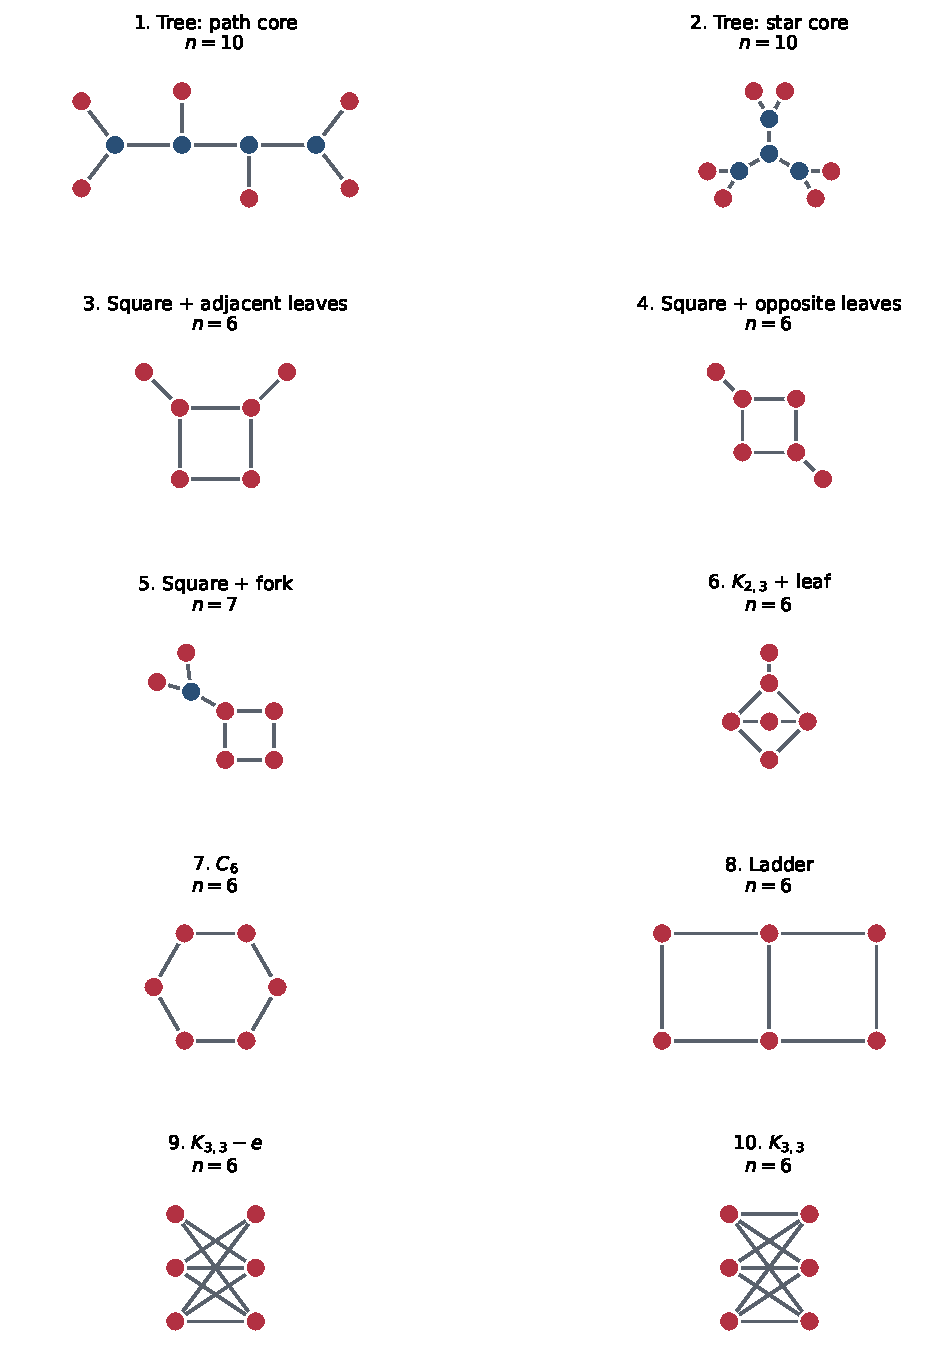
\includegraphics[width=\textwidth,height=.88\textheight,keepaspectratio]{figures/bipartite_six_kernels.pdf}
\caption{The ten bipartite subcubic six-boundary kernels. Boundary vertices
are red and interior vertices blue. Only bridges may be subdivided in this
construction; all such subdivisions are allowed. Unmarked edge crossings
are not vertices.}
\label{fig:bipartite-six-kernels}
\end{figure}

\subsection{Removing bipartiteness at boundary six}
The following section proves an all-orders reduction for nonbipartite
subcubic graphs as well, and then classifies the entire connected subcubic
six-boundary class. The bipartite theorem above remains stronger in another
direction: it applies to every boundary size and has a full graph-level
Lean proof.

For comparison, unrestricted two-connected searches at orders eight, nine,
and ten find respectively twelve, two, and one six-boundary graphs. The
last layer contains 9,743,542 graphs. This unrestricted census is only
finite evidence: the higher-degree six-boundary core problem remains open
in this work. These searches were made in the earlier session and are
not part of the package.

\section{Complete classification of subcubic six-boundary graphs}\label{sec:subcubic-six}
\begin{theorem}[Six boundary vertices, maximum degree three]\label{thm:subcubic-six}
There are exactly twelve two-connected subcubic graphs with six harmonic
boundary vertices: the ten two-connected subcubic graphs of order six,
the theta graph with path lengths $1,4,4$, and the subdivision of $K_4$
whose three edges in one triangle have length three and whose remaining
three edges have length one. In particular, their maximum order is ten.

Every connected subcubic graph with six harmonic boundary vertices is
obtained by arbitrary independent subdivisions of bridges of exactly one
of 201 reduced kernels. Their maximum order is eighteen, attained by
exactly two kernels. Both consist of four triangles joined by bridges,
with six additional leaves; the four triangle nodes induce $P_4$ or
$K_{1,3}$ in the contracted tree.
\end{theorem}
The new step is an all-orders structural proof for the interior of a
subcubic core. It turns a finite census into an exhaustive classification.
The subsequent block closure is independently certified without orbit
pruning.

\begin{figure}[p]
\centering
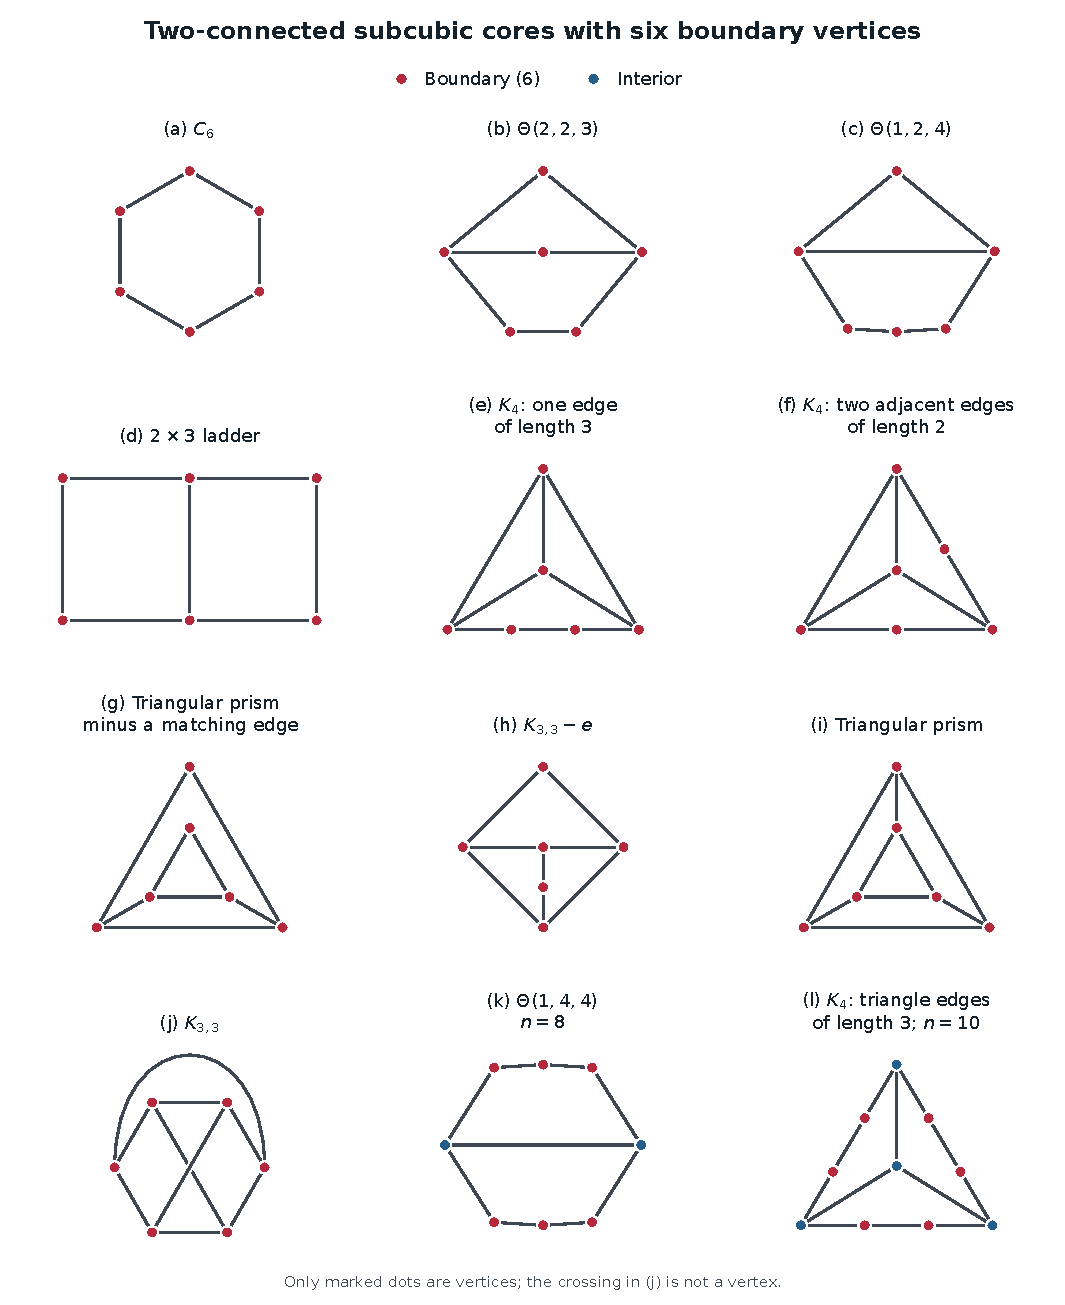
\includegraphics[width=\textwidth,height=.88\textheight,keepaspectratio]{figures/subcubic_twelve_cores.pdf}
\caption{The complete twelve-core subcubic six-boundary palette. The first
ten graphs have order six and all vertices boundary. The last two have
orders eight and ten. Red marks boundary vertices; blue marks interior
vertices. Every model is matched isomorphically to the exact catalogue and
checked by fresh integer shortest-distance calculations.}
\label{fig:subcubic-twelve}
\end{figure}

\subsection{The exact equations at an interior vertex}
Until the block-assembly step, let $G$ be two-connected and subcubic,
$B=\partial G$ with $|B|=6$, $I=V(G)\setminus B$, and $H=G[I]$.
Every vertex of $I$ has degree three in $G$: a degree-two vertex on a
cycle is boundary. The degree-three sector theorem gives independent
neighbors, a unique first neighbor towards each other target, and
exactly two boundary vertices in each of the three first-step sectors.
An edge of $H$ therefore has exactly two boundary coordinates increasing,
two decreasing, and two unchanged.

For a fixed $u\in I$, let its sectors be $S_v$, indexed by its neighbors.
Form a quotient graph $Q_u$ on the three neighbors, putting an edge
between $v,w$ when there is an edge between $S_v,S_w$ in $G-u$.
The quotient is connected. Put
\[
 P_v^w=\{x\in S_v:d(w,x)=d(u,x)\}.
\]
Then $P_v^w$ is nonempty exactly when $vw$ is an edge of $Q_u$.
One direction follows from a horizontal cross-sector edge. For the other,
a shortest $w$--$x$ path of length $r=d(u,x)$ starts at root level one
and ends at level $r$. If $n_-,n_0$ count its inward and horizontal steps,
then $2n_-+n_0=1$. Its sole horizontal step must cross directly from
$S_w$ to $S_v$, since vertical edges preserve sectors.

The sector-flux proof gives a boundary vertex in $P_v^w$ and one in
$S_v\setminus P_v^w$ whenever $P_v^w$ is nonempty. To recall the sign
argument, edges leaving the first set are nonincreasing in distance
from $u$, with at least one strictly decreasing; summing scores cancels
internal edges. For the complement use distance from $w$, with the
strict edge $vu$. Because $S_v$ has exactly two boundary points, precisely
one lies in each set.

If a neighbor $w$ of $u$ is interior, the edge $uw$ has two horizontal
boundary coordinates. Their number equals $\deg_{Q_u}(w)$, so this degree
is two. If a neighbor $v$ is boundary, it belongs to none of the sets
$P_v^w$, since independent root neighbors give $d(w,v)=2$. Quotient
degree two would place its sole sector-mate in both such sets, giving
one closer and two equidistant neighbors at $u$ and hence a positive
score. Thus boundary neighbors have quotient degree one. The connected
quotient is consequently $P_3$ or $K_3$, and
\begin{equation}\label{eq:subcubic-H-degree}
 \deg_H(u)\in\{1,3\}.
\end{equation}
In particular, an $H$ leaf has exactly two boundary neighbors, and an
internal $H$ vertex has none. Also $|I|$ is even.

Let $F(x)=\sum_{b\in B}d(x,b)$. It is constant on each $H$ component.
For an edge from $u\in I$ to $v\in B$, the six changes consist of two
$-1$'s, one zero, and three $+1$'s, so $F(v)=F(u)+1$.
At an internal $H$ vertex, the six nonpositive scores sum to zero.
At an $H$ leaf, their sum is $-2$ and each of its two adjacent boundary
targets gives score $-1$. Hence
\begin{equation}\label{eq:subcubic-exact-score}
 \boxed{\stab_G(u,b)=-\ind_{u\sim b}\qquad(u\in I,\ b\in B).}
\end{equation}
Equivalently, $x\mapsto d(x,b)-\ind_{x=b}$ is harmonic at every interior
vertex. This exact equality is stronger than the defining nonpositive
inequality and is the source of the reduction below.

\subsection{Propagation of tight boundary pairs}
The boundary profiles satisfy
\[
 d(x,y)=\max_{b\in B}|d(x,b)-d(y,b)|,
 \qquad \forall b\ \exists c:\ d(x,b)+d(x,c)=d(b,c).
\]
These properties also follow directly by extending a geodesic away from
its initial target while its endpoint is nonboundary. A nonboundary
endpoint has a farther neighbor, since it has a closer one and nonpositive
score. Strictly increasing distance forces the extension to terminate
at a boundary vertex.

There is no five-cycle in $H$. For each boundary coordinate its horizontal
edges form a matching: two horizontal neighbors would leave one closer
neighbor and give positive score. On a five-cycle the horizontal count is
odd and at most two, hence one. Six coordinates would give six horizontal
edge incidences, while the five edges of $H$ each contribute two, giving
ten. This is impossible.

At an internal $H$ vertex $u$, suppose $b,c$ form a tight pair. Its
nonnegative defect
\[
 g_{bc}(x)=d(x,b)+d(x,c)-d(b,c)
\]
has value zero at $u$. Equation~\eqref{eq:subcubic-exact-score} implies
$\sum_{x\sim u}g_{bc}(x)=0$, so the pair remains tight at every neighbor.
Every coordinate has increments $-1,0,1$ at $u$, and each incident edge is
horizontal in exactly two boundary coordinates. A tight partner must have
the same horizontal edge. Thus the six coordinates are partitioned into
three unique tight pairs. This perfect matching agrees across an edge
between two internal $H$ vertices.

Consider such an edge $uv$, with other neighbors $x,y$ of $u$ and $p,q$
of $v$. On all these vertices, the paired coordinates are complementary.
Select one coordinate from each pair, translate, permute, and reverse
coordinate signs. The exhaustive normal form is
\[
 u=(0,0,0),\quad v=(0,1,1),\quad
 x=(1,0,-1),\quad y=(-1,-1,0),
\]
\[
 p=(\varepsilon,1,2),\quad q=(-\varepsilon,2,1),
 \qquad\varepsilon\in\{-1,1\}.
\]
Both sign cases give $d(y,p)=d(x,q)=2$ by profile isometry.
A common neighbor of $y,p$ cannot be $u,v$ or an interior vertex: the
first choices create a triangle through an interior vertex, and the last
creates a five-cycle $yuvpw$ in $H$. It is therefore boundary. By
\eqref{eq:subcubic-H-degree}, $y,p$ are $H$ leaves. The same holds for $x,q$.
Every internal-to-internal edge therefore exhausts a six-vertex double-star
component. Consequently
\[
 H\text{ has only components }K_2,\ K_{1,3},\text{ or a six-vertex double-star}.
\]
If $\ell$ is its number of leaves, then $|I|\le3\ell/2$ and $|I|$ is even.
Since $2\ell=|E(I,B)|\le18$, this already proves the unconditional
finite bound $|V(G)|\le18$.

\subsection{A sharper hand reduction to order fourteen}
The double-star can in fact be excluded without enumeration. If
$\varepsilon=1$, every selected-coordinate difference between $y,p$ has
absolute value two, as do the complementary differences. A common boundary
neighbor would have distance one from both and hence give a zero difference,
a contradiction.

Suppose $\varepsilon=-1$. Write the actual coordinate values at $u$ as
$D_1,D_2,D_3$ and their complementary values as $D'_1,D'_2,D'_3$.
A boundary neighbor $w$ common to $y,p$, and a boundary neighbor $z$ common
to $x,q$, must be the two endpoints of pair one, forcing
$D_1=D'_1=2$. Positivity on the six interior vertices gives
\[
 D_2,D_3\ge2,\qquad D'_2,D'_3\ge3.
\]
Each $H$ leaf needs a second boundary neighbor. The only coordinate
that can equal one forces respectively
\[
 x\sim c,\quad y\sim a,\quad p\sim c',\quad q\sim a',
 \qquad D_2=D_3=2,\quad D'_2=D'_3=3,
\]
where $(a,a')$ and $(c,c')$ are pairs two and three.
Now $d(x,a)=2$. Among $x$'s neighbors $u,z,c$, the first has distance two
from $a$, and $d(z,a)\ge3$ because $z\sim q$ and $d(q,a)=4$.
Therefore $c\sim a$. The symmetric argument at $p$ forces $c'\sim a'$.
But $d(x,c')=4$, while the distances to $c'$ from $x$'s three neighbors
are $3,5,$ and at most three: the last bound follows from $zqa'c'$.
Thus $\stab_G(x,c')\ge12-(3+5+3)=1$, a contradiction.
We have proved that $H$ has only edge and three-leaf-star components.

There is at most one star component and it precludes every other component.
Its three leaves have distinct boundary neighbors: a shared boundary point
would give two length-two geodesics between interior leaves. Hence its center
has boundary profile $(2,2,2,2,2,2)$. Two centers would violate injectivity.
For a separate edge component $uv$, its four boundary neighbors are distinct.
The two missing boundary coordinates have equal values $r,s$ at $u,v$.
Equation~\eqref{eq:subcubic-exact-score} makes the corresponding distances
from the two boundary neighbors of $u$ equal $r-1,r+1$, and similarly for
$s$. The star center implies that all boundary distances are at most four,
so $r,s\le3$. Every coordinate of $u$ is now between one and three, putting
it at sup-distance at most one from the star center. That would make the
two components adjacent, a contradiction.

Thus either $H=K_{1,3}$ and $|V(G)|=10$, or $H$ is a matching of at most
four edges, because each edge component uses four incidences at the six
boundary vertices. In all cases
\[
 \boxed{|V(G)|\le14.}
\]
An independent standard-library BFS checker exhausts all 60,070
isomorphism classes of two-connected subcubic graphs on orders six through
fourteen, generated by nauty. Exactly twelve have boundary six, and they
are precisely the cores in Theorem~\ref{thm:subcubic-six}. The larger census
through order eighteen, made in the earlier session, is a separate
corroboration. The order bound is proved before either census is used.
The census through order fourteen was repeated without nauty for this
release (Section~\ref{sec:verification}).

\subsection{Exact block assembly and the 201 kernels}
At intrinsic boundary at most five, every two-connected subcubic block is
all boundary, by the degree-three obstruction. Its order is at most five.
The full palette therefore consists of all two-connected subcubic graphs
on three through six vertices, and the exceptional cores of orders eight
and ten: twenty nonbridge types in total.

Distinct nonbridge blocks of a subcubic graph are vertex-disjoint. Bridges
attach only at intrinsic degree-two block vertices, at most one per vertex.
At such a vertex the intrinsic stability is one or two; one external bridge
lowers it by one. Let $h_C$ count attached sites of intrinsic stability one,
and let $L$ count ordinary leaves outside the blocks. The exact assembly
condition is
\begin{equation}\label{eq:subcubic-six-assembly}
 6=L+\sum_C\bigl(b(C)-h_C\bigr).
\end{equation}
Choose any block tree from the palette, with ordinary vertices of degrees
one or three, attach its bridges injectively to available degree-two sites,
and impose \eqref{eq:subcubic-six-assembly}. Together with arbitrary bridge
subdivision, this is a necessary-and-sufficient constructive description.

For the reduced-order bound, write $R=\sum_C(b(C)-2)$ and let $\Delta_*\ge0$
be the total cut defect in the exact block budget. Then $R+\Delta_*=4$.
Every palette block satisfies $|V(C)|\le3(b(C)-2)$, with equality only for
a triangle. If $A$ counts ordinary degree-three vertices, each contributes
at least one cut defect, so $A\le\Delta_*$. Since $L\le6$,
\[
 |V(K)|=\sum_C|V(C)|+A+L
 \le3R+\Delta_*+6=18-2\Delta_*\le18.
\]
Equality forces four triangles, six ordinary leaves, no ordinary branch
vertex, and every triangle site buried by a bridge. The contracted tree
has four trivalent internal nodes, whose induced tree is $P_4$ or
$K_{1,3}$. These give exactly the two equality kernels.

\begin{figure}[p]
\centering
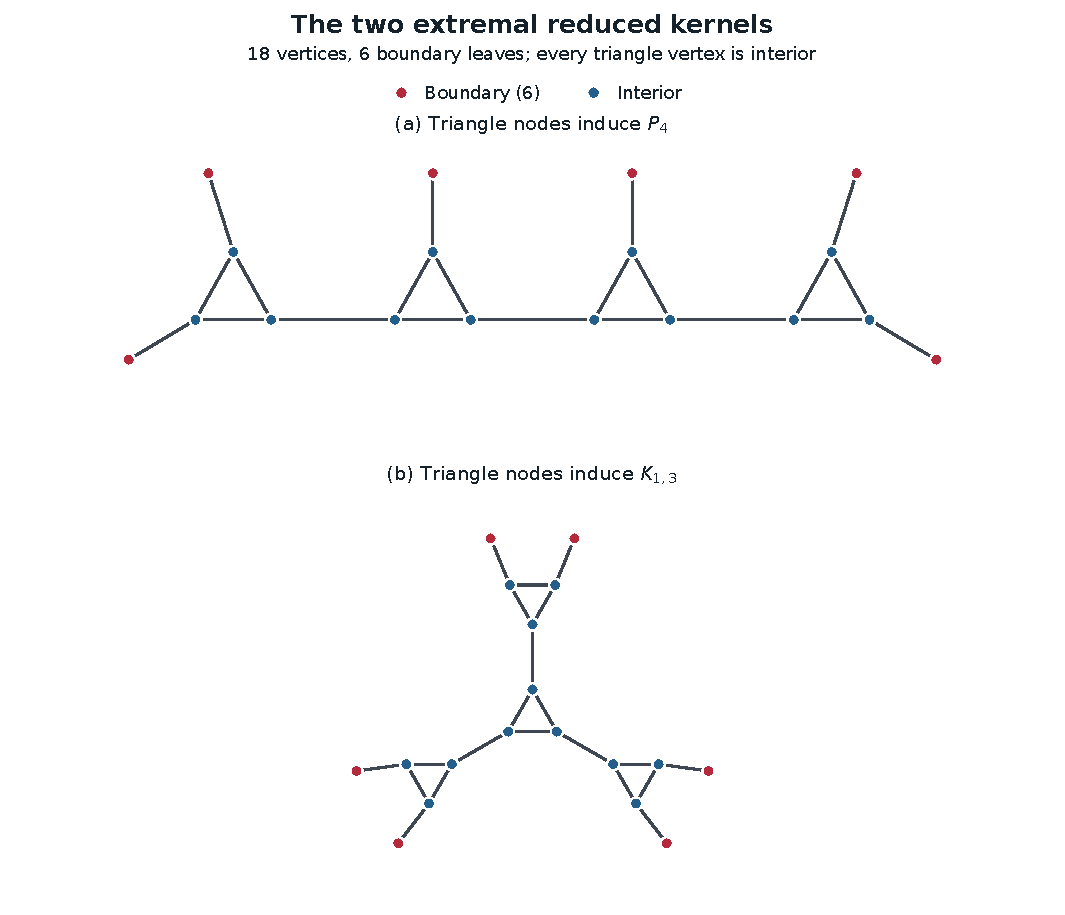
\includegraphics[width=\textwidth]{figures/subcubic_extremizers18.pdf}
\caption{The two eighteen-vertex reduced kernels attaining the sharp
subcubic six-boundary bound. Their boundary consists of the six leaves.
Arbitrary subdivisions of the displayed bridges preserve the boundary.}
\label{fig:subcubic-extremizers}
\end{figure}

The finite closure uses rooted block attachment and insertion of a new
trivalent branch on a bridge, retaining maximum degree three and boundary
at most six. The usual end-block induction proves completeness. There
are 264 states of boundary at most six, of which 201 have boundary six.
Their order distribution is
\begin{center}\small
\begin{tabular}{@{}rrrrrrrrrrrrrr@{}}\toprule
$n$&6&7&8&9&10&11&12&13&14&15&16&17&18\\\midrule
Number&16&8&10&9&23&20&32&25&27&15&11&3&2\\\bottomrule
\end{tabular}
\end{center}
The independent verifier imports no generator and uses no orbit pruning.
It checks all 47,332 degree-admissible vertex/root attachments, all 1,257
bridge branchings, fresh boundary scores and reducedness for every state,
well-founded generation of every nonseed, and exact canonical closure.
The 63 states with boundary at most five agree exactly with the previous
subcubic catalogue. The whole subcubic six-boundary proof is not claimed
to be formalized in Lean; its sector input is formalized, its new reductions
are conventional proofs, and its finite catalogues have exact
reproducible checkers.

\section{An infinite obstruction to purely local six-boundary tests}\label{sec:six-local-barrier}
The general rooted reduction does not settle global compatibility. The
following theorem makes the obstruction explicit, at unbounded diameter.
The local model here is exactly the radius-two induced-frame model with
minimum degrees, harmonic inequalities, all selected-target descents, and
the two-path condition used in the experimental extension.

\begin{theorem}[All-root local feasibility does not imply realizability]
For each integer $t\ge3$, let $M_t$ be the metric on
$A=\{a_1,a_2,a_3\}$ and $B=\{b_1,b_2,b_3\}$ with
\[
 M_t(a_i,b_j)=t,\qquad
 M_t(a_i,a_h)=M_t(b_i,b_h)=2t-1\quad(i\ne h).
\]
At every designated root, $M_t$ has a feasible radius-two local model
satisfying all the conditions just listed, including every nonpositive
interior score toward every designated or selected local target.
Nevertheless, no finite simple connected graph has exactly these six
harmonic boundary vertices with boundary metric $M_t$.
\end{theorem}
\begin{proof}
First describe its entire positive profile frame. Each part has a unique
coordinate at most $t-1$. Otherwise its coordinates could have no tight
partner; two such small coordinates would violate their sum inequality.
Write the small coordinates as $a$ at $a_i$ and $b$ at $b_j$. Every other
coordinate in its part must be at least $2t-1$ minus that minimum. It is
therefore at least $t$, so it cannot have a cross-part tight partner. Its
only possible tight partner is its own part's minimum. Thus every positive
profile is exactly
\[
 \begin{array}{ll}
 p(a_i)=a,&p(a_h)=2t-1-a\quad(h\ne i),\\
 p(b_j)=b,&p(b_h)=2t-1-b\quad(h\ne j),
 \end{array}
 \qquad 1\le a,b\le t-1,\quad a+b\ge t.
\]
Denote this profile by $p(i,j;a,b)$. Conversely each displayed profile
satisfies all frame conditions.

At root $a_i$, select the root and the six profiles
\[
 p(i,j;1,t-1),\quad p(i,j;2,t-2)\qquad(j=1,2,3).
\]
They induce a $K_4$ on the root and its three first-step vertices, with one
pendant second-step vertex at each first-step vertex. The root degree is
three and the three constrained interior degrees are four. There are
three disjoint layer-one to layer-two edges. For the first-step vertex
indexed by $j$, its scores toward $a_i$, any other $a_h$, $b_j$, and any
other $b_h$ are respectively $0,0,-2,0$. Toward the selected local vertices,
the only negative scores are at itself and its own pendant, and all other
scores are zero. Every target has a closer selected neighbor. The
six-sector rule for degree-three interiors is vacuous. Symmetry gives a
valid model at all six roots, uniformly in $t$.

Suppose a graph realizing this exact boundary exists. Its distance profiles
form an isometric induced subgraph of the full frame. A length-$t$ geodesic
from $a_i$ to $b_j$ forces every profile $p(i,j;k,t-k)$,
$1\le k\le t-1$: at its $k$th step both endpoint distances are below $t$,
so they are the unique small coordinates. Hence every diagonal profile
$a+b=t$ is present.

Consider such a forced profile with $a=k\le t-2$, and its score toward
$a_h$ with $h\ne i$. Its predecessor on the diagonal, or $a_i$ when $k=1$,
contributes $-1$; its forced successor contributes $+1$. For $k>1$, the
only possible additional positive contributors are profiles with
coordinates $(k+1,t-k)$ or $(k+1,t-k+1)$; the profile $(k,t-k+1)$, if
present, contributes zero. At $k=1$, the other first-step vertices also
contribute zero, while all the profiles $p(i,j';2,t-1)$ contribute $+1$.
An interior score cannot be positive. Thus every additional positive
contributor is absent. Applying this at all diagonal profiles deletes the
entire two layers $a+b=t+1$ and $a+b=t+2$.

Every profile edge changes $a$ and $b$ by at most one. If an index changes,
the corresponding two small coordinates must both equal $t-1$, which
also respects that bound. Designated points meet only diagonal profiles.
The two missing layers therefore separate every higher profile from the
boundary. Connectivity excludes all higher profiles, leaving precisely
the six designated points and the forced diagonals.

This remaining graph consists of six $K_4$ clusters, with ports
$P_{ij}$ at the $A$ side and $Q_{ij}$ at the $B$ side, joined by nine
internally disjoint chains of length $L=t-2$. For $i\ne i'$ and $j\ne j'$,
\[
 \|P_{ij}-Q_{i'j'}\|_\infty=t-1,
 \qquad d(P_{ij},Q_{i'j'})=t.
\]
Indeed, using one chain requires a turn in each endpoint cluster, for a
total of $L+2=t$, and this is attained. Any other route uses at least
three chains and costs at least $3L\ge L+2$. The discrepancy contradicts
isometry of the boundary-profile embedding. This proves the impossibility
for every $t\ge3$.
\end{proof}

The positive frame has $9t(t-1)/2$ profiles; the forced diagonal graph has
$9t-3$ vertices. The smallest member was found by a local metric search;
its full 33-vertex frame is also independently rejected by an SMT model.
The theorem's proof is the uniform argument above, not that solver result.
The standard-library checker regenerates the full frame directly for
$t=3,4,5$, checks local score coefficients and layer exclusions for
$3\le t\le12$, and checks the final distance discrepancy by fresh BFS.
This identifies a precise limitation of the existing local model, rather
than extrapolating a six-boundary classification from small graphs.

\begin{corollary}[The same local obstruction at every larger boundary size]
For every $k\ge6$ there are integer metrics on $k$ designated points, of
unbounded diameter, which pass all the specified radius-two local tests
at every root but cannot be harmonic boundary metrics of any connected graph.
\end{corollary}
Indeed, use parts of sizes $p,q\ge3$ with $p+q=k$, cross distances $t$ and
within-part distances $2t-1$. The same profile, layer, and isometry arguments
apply. At an $A$-root the local model is a $K_{q+1}$ with a pendant
second-step vertex at each nonroot vertex. Its first-layer interior degrees
are $q+1\ge4$. The score toward the matching opposite target is $1-q$;
the other designated-target scores are zero. The symmetric description
holds at a $B$-root. Thus the local witnesses meet the same constraints,
while the two missing layers force the same global distance discrepancy.


\section{Verification, dependencies, and further questions}\label{sec:verification}
\subsection{Exact computational scope}
All finite decisions use integer breadth-first distances and integer
stability sums. The package directory \texttt{checks/} contains the
checkers and data used below; \texttt{checks/run\_checks.py} replays them
in a temporary copy. The checks needed by the proofs are: the exact
inverse matrices of the three cones; the capped local certificate, with
its 835 contradiction trees, 306 feasible selections and a regeneration
of all 1,613,472 coefficient choices; the fifteen residual metrics; the
complete block palette through order six; the 227-kernel closure; and,
for the extensions, the grammar closures, counting identities and audits
cited in their sections. The subcubic core census and the 201-kernel
closure were carried out with nauty~2.8.9 \cite{nauty}; their checkers
are included and run when the nauty programs are supplied.

The following enumerations were written independently for this release
and share no code with the other checkers. Graphs were generated by adding
vertices (or, for two-connected graphs, ears) and deduplicated by exact
isomorphism tests.
\begin{itemize}
\item Every connected graph of order at most eight with five boundary
vertices reduces to one of the 119 catalogue kernels of order at most
eight, and every such kernel occurs.
\item Every connected subcubic graph of order at most eleven with six
boundary vertices reduces to one of the 86 catalogue kernels of order at
most eleven, and every such kernel occurs.
\item At orders $6,\dots,14$ the numbers of two-connected graphs of
maximum degree at most three are $10$, $18$, $49$, $115$, $349$, $1011$,
$3421$, $11679$ and $43418$; these
60,070 graphs agree with the nauty census, and exactly twelve of them,
the cores of Theorem~\ref{thm:subcubic-six}, have six boundary vertices.
\item Starting from the two-connected blocks with boundary at most six
found by that census, and from $K_2$, the attachment closure of
Theorem~\ref{thm:227} produces exactly 264 subcubic reduced graphs with
boundary at most six, of which exactly 201 have boundary six; they are
the catalogue. The same closure started from all two-connected graphs of
order at most six with boundary at most five produces 264 reduced graphs,
of which exactly 227 have boundary five; they are the catalogue.
\item For $n\le13$, the minimum boundary of an $n$-vertex two-tree and the
number of minimizers agree with Theorem~\ref{thm:twotree} and with the
counts $2,7,3,18,3,36,3,66$ at $n=6,\dots,13$ given by
Section~\ref{sec:exact-odd-count}.
\end{itemize}
These enumerations check the catalogues and the implementations; the
order bounds that make the catalogues complete are the proved theorems.

\subsection{Formal verification: precise scope}
The Lean project in \texttt{lean/} uses Lean~4.35.0 and its standard
library; it pins Mathlib for uniformity with the other projects of this
repository but imports none of it. The audit module
\texttt{HarmonicBoundary.AxiomAudit} enumerates every declaration defined
in the project modules (15,771 declarations, including generated ones)
and checks that each depends only on \texttt{propext},
\texttt{Classical.choice} and \texttt{Quot.sound}. There is no
\texttt{sorry}, no added axiom and no \texttt{native\_decide}; finite facts
are proved by kernel-checked \texttt{decide} or \texttt{omega}.
\begin{itemize}
\item \texttt{DistanceCertificate} defines walks of a given length and
proves that a table satisfying local conditions is the shortest-walk metric.
\item \texttt{RootSectors} proves Theorem~\ref{thm:degree3} at graph level:
from a finite simple graph, certified distances, a nonboundary vertex of
degree three and connectivity after deleting it, it constructs a
duplicate-free list of six boundary vertices.
\item \texttt{WedgeDistance} and \texttt{WedgeBoundary} prove the distance
and stability formulas for a one-point union of two graphs, the binary case
of Theorem~\ref{thm:block}. \texttt{BlockBudget} proves the accounting
identity and the kernel bounds from an explicit accounting record; it does
not construct the block-cut tree.
\item \texttt{Sharp14} certifies the distances of Figure~\ref{fig:sharp} and
that exactly vertices 9--13 are boundary.
\item The 42 modules \texttt{LocalSystems/} state and prove the 835 local
infeasibility systems of Section~\ref{sec:capping}, each with its Boolean
bounds, degree and score inequalities and two-path condition written in the
statement. The link between these statements and the profile certificate is
made by the certificate checker, not in Lean.
\item \texttt{RootedMetricTruncation} proves the rooted metric theorem of
Section~\ref{sec:rooted-truncation}, with both sharp constants, on an
arbitrary index type; \texttt{BipartiteSubcubic} proves the boundary
characterization of Section~\ref{sec:bipartite-subcubic} at graph level.
\item \texttt{EvenEqualityAutomaton} and \texttt{OddEqualityGrammar} prove
the weight bounds for all runs and derivations of the two-tree grammars,
and the degree bound six; \texttt{OddCountingIdentities} proves the
polynomial identities behind the counting formula. The correspondence
between graphs and grammar derivations is a conventional proof.
\end{itemize}
The metric-cone coverage, the capping reduction, the diameter-three
argument, the general block decomposition, the two-tree charging argument,
the subcubic interior reduction and the catalogue enumerations are not
formalized.

\subsection{Rejected shortcuts and remaining extensions}
Two tempting reductions are false. A theta graph with three internally
disjoint terminal paths of lengths $1,4,4$ has boundary six and diameter four,
so a proposed general bound $b(G)\ge2\diam(G)$ for two-connected graphs fails.
Also, take a pentagon with leaves attached at three vertices, two of them
adjacent. The endpoints of the edge joining those two vertices are interior.
Contracting that edge
produces a square and increases boundary five to boundary six. An explicit
adjacency certificate is included. Thus arbitrary interior-edge contraction
cannot justify the finite core bound.

The former unbounded-diameter obstruction is closed by
Theorem~\ref{thm:unrestricted}. The large order and diameter searches are
independent audits and discovery tools; they are not needed to justify
unbounded completeness. The essential finite dependency is the capped
local certificate. The small residual metrics have hand exclusions.

The previous open equality cases in the two-tree bound are now closed by
Section~\ref{sec:two-tree-equality-new}; Section~\ref{sec:exact-odd-count}
gives the exact unlabelled count at every order. The complete connected
subcubic six-boundary classification is proved in
Section~\ref{sec:subcubic-six}, including the sharp order bound and both
equality kernels. Sections~\ref{sec:rooted-truncation} and
\ref{sec:bipartite-subcubic} give all-radius and all-boundary-size extensions.
The stated radius-two approach has a proved global compatibility limitation
at every boundary size at least six, by Section~\ref{sec:six-local-barrier}.

The remaining limits are specific. Six-boundary graphs having maximum degree
at least four are not classified here; no general order bound for their
two-connected cores is proved. The exact block budget reduces that question
to the missing core palette. The complete five-boundary
graph-to-cone-to-kernel chain, the new subcubic six-boundary classification,
and the two-tree graph-to-grammar and unlabelled-counting correspondences
are not formalized end to end in Lean. At every fixed two-tree excess,
rational unlabelled enumeration is proved by a terminating finite procedure;
explicit simplified formulas for $e\ge2$ are not computed here, and no
general quasipolynomial or polynomial-growth assertion is made. The metric truncation theorem
preserves the specified neighborhoods about one chosen root; simultaneous
all-root compatibility is a distinct question. No external peer review
or exhaustive priority claim is made.

\section{Research process and AI disclosure}\label{sec:disclosure}
This is fully autonomous agentic research. The results, their proofs, the
finite certificates and checkers, the original Lean development and the
literature search were produced by autonomous AI research agents in an
earlier session; its records do not name the system used. The audits
described in those records were carried out within the same automated
workflow.

Opus~5.5 by Anthropic used with Claude Code assessed the work for this
release. It identified the source problem in the paper of Chiem, Dudarov,
Lee, Lee and Liu, read the proofs of the diameter theorem, the capping
reduction and the subcubic interior reduction, reran the checkers listed
in the previous section, wrote and ran the independent enumerations listed
there, arranged the Lean files as one project with a whole-project axiom
audit, ran the fresh build, and edited this manuscript. The nauty-based
census and closure were not rerun with nauty; the independent census and
closure replace them in this release. The remaining sections were carried
over and read, but not all were rederived line by line.

Dev D. Goyal is responsible for publication. The work has not been
externally peer reviewed; AI checks are not human peer review, no expert
validation is claimed, and the literature comparison is bounded and does
not establish priority.

\clearpage
\begingroup\small\setlength{\parskip}{0pt}
\begin{thebibliography}{99}\setlength{\itemsep}{2pt}
\bibitem{chiem}
N. Chiem, W. Dudarov, C. Lee, S. Lee, and K. Liu,
\emph{A characterization of graphs with at most four boundary vertices},
Journal of Combinatorics 15(3) (2024), 361--382.
\href{https://arxiv.org/abs/2209.04438}{arXiv:2209.04438v2};
\href{https://doi.org/10.4310/JOC.240907013024}{doi:10.4310/JOC.240907013024}.
\bibitem{steinerberger2022}
S. Steinerberger, \emph{The boundary of a graph and its isoperimetric inequality},
Discrete Applied Mathematics 338 (2023), 125--134.
\href{https://arxiv.org/abs/2201.03489}{arXiv:2201.03489}.
\bibitem{steinerberger2025}
S. Steinerberger, \emph{Potential theory and the boundary of combinatorial graphs},
2025. \href{https://arxiv.org/abs/2507.20833}{arXiv:2507.20833v1}.
\bibitem{muller}
T. M\"uller, A. P\'or, and J.-S. Sereni,
\emph{Graphs with four boundary vertices},
\href{https://www.math.rug.nl/~tobias/Papers/boundary4.pdf}{author-hosted paper}.
\bibitem{koolen}
J. H. Koolen, A. Lesser, and V. Moulton,
\emph{Optimal realizations of generic five-point metrics},
European Journal of Combinatorics 30 (2009), 1164--1171.
\href{https://doi.org/10.1016/j.ejc.2008.09.021}{doi:10.1016/j.ejc.2008.09.021}.
\bibitem{celik}
D. \c{C}elik, \emph{Explicit determination of Gromov-product types of
five-point metric spaces}, Eski\c{s}ehir Technical University Journal of
Science and Technology B 6(2) (2018), 185--192.
\href{https://doi.org/10.20290/aubtdb.375635}{doi:10.20290/aubtdb.375635}.
\bibitem{nauty}
B. D. McKay and A. Piperno, \emph{nauty and Traces}, version 2.8.9.
\href{https://users.cecs.anu.edu.au/~bdm/nauty/}{Maintainer distribution and documentation}.
\end{thebibliography}
\endgroup
\end{document}
